% alibz manuscript — arXiv preprint; journal target: Applied Spectroscopy (SAS/SAGE).
% Build: make   (latexmk -pdf).  Switch \arxivtrue/\arxivfalse below for journal layout.
\documentclass[11pt]{article}

\newif\ifarxiv
\arxivtrue

\usepackage[utf8]{inputenc}
\usepackage[T1]{fontenc}
\usepackage{lmodern}
\usepackage{microtype}
\usepackage{amsmath,amssymb,mathtools}
\usepackage{graphicx}
\usepackage{booktabs}
\usepackage{siunitx}
\usepackage{xcolor}
\usepackage[numbers,sort&compress]{natbib}
\usepackage[margin=1in]{geometry}
\usepackage{lineno}
\usepackage[colorlinks=true,allcolors=blue]{hyperref}
\usepackage{orcidlink}
\usepackage{authblk}

\sisetup{range-phrase=--, range-units=single, per-mode=symbol}
\graphicspath{{figures/}}

% ---- editorial macros ----
\newcommand{\todo}[1]{\textcolor{red}{[TODO: #1]}}
\newcommand{\alibz}{\texttt{alibz}}
\newcommand{\nel}{n_{\mathrm{e}}}
\newcommand{\kB}{k_{\mathrm{B}}}
\newcommand{\Tex}{T}
\newcommand{\order}[1]{\mathcal{O}(#1)}
\DeclareMathOperator*{\argmin}{arg\,min}

\ifarxiv
  \linenumbers
\fi

\title{Calibration-free quantification of laser-induced breakdown spectra by
  whole-pattern forward modelling: theory, assumptions, workflow, datasets and
  fit metrics behind \alibz}

\author[1,2]{Michael L. Whittaker\thanks{Corresponding author: mwhittaker@lbl.gov}}
\affil[1]{Energy Geosciences Division, Lawrence Berkeley National Laboratory, Berkeley, CA 94720, USA}
\affil[2]{Materials Sciences Division, Lawrence Berkeley National Laboratory, Berkeley, CA 94720, USA}
\date{\today}

\begin{document}
\maketitle

\begin{abstract}
Laser-induced breakdown spectroscopy (LIBS) can in principle quantify elemental
composition without matrix-matched standards by inverting a physical model of
the plasma emission, the calibration-free (CF-LIBS) programme. In practice the
inversion is ill-posed: temperature, electron density, optical depth, detector
response and line identification are entangled, and small errors in any one
appear as large, self-consistent errors in composition. This paper sets out the
theoretical basis, the explicit assumptions, the processing workflow, the
datasets and the fit metrics that underpin \alibz, an open-source toolkit that
treats a LIBS spectrum as a non-negative linear combination of forward-modelled
element--ion templates evaluated at a shared plasma state, and solves the
inverse problem with physical constraints rather than empirical calibration
curves. We describe the local-thermodynamic-equilibrium emission model and its
conventions, the treatment of self-absorption by resolved-profile and
doublet-ratio inversion, the electron-density anchors, the stage-consistency
thermometer that fixes temperature where the amplitude data cannot, the
peak-extraction and refinement pipeline, the whole-pattern weighted
non-negative solve with its evidence terms and basin guards, and the
true-negative contest that resolves spectral confounders. We define the
diagnostics by which a fit is judged, report where the method currently
succeeds and fails on synthetic and real spectra from a handheld analyser, and
state the validation gates that remain open: composition invariance between
argon and air, pure-element standards for the plasma physics, and certified
reference materials for the composition solve.
\end{abstract}

\noindent\textbf{Keywords:} laser-induced breakdown spectroscopy; calibration-free
LIBS; Saha--Boltzmann; self-absorption; non-negative least squares; spectral
unmixing; handheld LIBS

\section{Introduction}
\label{sec:intro}

Laser-induced breakdown spectroscopy (LIBS) determines elemental composition from the atomic and ionic emission of a microplasma produced by a focused, pulsed laser.
The technique needs no sample preparation, works in air at standoff or contact, and records most of the periodic table in a single shot, which explains its adoption across metallurgy, environmental monitoring, geochemistry, and planetary exploration \citep{hahn2010review1,hahn2012libs,fortes2013libs,cremers2013handbook}.
Turning a spectrum into a mass fraction is nonetheless difficult.
The emitted intensity depends on the amount of ablated mass, which varies with laser coupling and sample physical state \citep{russo2013ablation}; on the plasma temperature and electron density, which evolve in time and space and differ from shot to shot \citep{aguilera2004spatial,borduchi2022detection}; and on the ambient gas \citep{palasti2022argon}.
Matrix effects couple these factors to the bulk composition and structure of the target, so that the same element at the same concentration yields different line intensities in different hosts \citep{eppler1996matrix,takahashi2017matrix}.
Strong lines are further distorted by self-absorption, which flattens and broadens them and biases both intensity ratios and concentration estimates \citep{bulajic2002selfabsorption,palleschi2022selfabsorption}.
Finally, the measured spectrum is the product of the plasma emission and the wavelength-dependent response of the spectrometer and detector, which must be known to compare lines far apart in wavelength \citep{li2014spectralresponse}.

Two families of calibration strategy have been developed to cope with these effects.
The first is empirical: spectra from reference materials of known composition are used to build univariate calibration curves, or multivariate models such as partial least squares (PLS) regression, that map intensities to concentrations \citep{clegg2009pls,dyar2016univariate,costa2021calibration}.
These models can be accurate within the compositional range of their training set, and the ChemCam and SuperCam programs have refined them over more than a decade \citep{wiens2012chemcam,anderson2017submodels,wiens2021supercam,anderson2022supercam}.
Their weakness is that they are interpolative.
Univariate curves are valid only for matrix-matched standards, and multivariate models degrade when the unknown differs from the training set in composition, physical state, or instrument condition \citep{dyar2016univariate,eppler1996matrix}.
Certified reference materials exist for common glasses, rocks, and alloys \citep{jochum2005georem,jochum2011nist}, but they cover only a small part of natural compositional space, and the limit of quantification one obtains depends on that coverage \citep{mermet2008loq}.
The second family is calibration-free LIBS (CF-LIBS).
Introduced by \citet{ciucci1999cflibs} and reviewed by \citet{tognoni2010cflibs}, it assumes that the plasma is optically thin, stoichiometric with the sample, and in local thermodynamic equilibrium (LTE), so that Boltzmann and Saha relations link line intensities to the temperature, electron density, and species populations \citep{cristoforetti2010lte,aguilera2007multielement}.
Composition then follows from a plasma-state fit and a closure condition, without reference spectra.
The same assumptions are the method's known failure modes.
Departures from LTE, spatial and temporal gradients, unresolved or unmeasured ion stages, and self-absorption all bias the inferred state \citep{cristoforetti2010lte,cristoforetti2013columnar,aguilera2004spatial}.
Accuracy on oxide and alloy targets has been reported to depend strongly on the line selection and on corrections applied to the data \citep{praher2010cflibs,herrera2009cflibs}.
Several refinements address individual weaknesses: internal reference and iterative corrections for self-absorption \citep{bulajic2002selfabsorption}, curve-of-growth and $C\sigma$ approaches that retain optically thick lines \citep{aragon2014csigma,aragon2015generalizedcog}, one-point calibration that borrows a single standard to absorb unknown scale factors \citep{cavalcanti2013onepoint}, radiative-transfer and Monte Carlo plasma models \citep{gornushkin2022montecarlo}, and statistical definitions of detection limits suited to the method \citep{villasboas2023lod}.
Direct tests of optical thinness, for example by branching ratios, are available but are applied to few lines at a time \citep{urbinamedina2021branching}.

Machine learning (ML) is the third approach and is now the most active.
Reviews catalog its use for classification, regression, and line identification \citep{hao2024mlreview,dehbozorgi2025mldl,zhang2023dlreview}.
Compared with linear calibration, regularized and nonlinear regressors, artificial neural networks, and convolutional networks cope better with nonlinear response and matrix effects when sufficient training data are available \citep{sirven2006ann,li2020cnn}.
Transfer learning and calibration sharing reduce the data demand when moving between instruments \citep{kepes2022transfer,lepore2024calsharing}, and shared benchmark datasets make methods comparable \citep{kepes2020benchmark}.
Line identification has itself been automated \citep{noel2025alias}.
What these methods do not provide is equally clear.
A trained network is an interpolator in the space of its training spectra; it carries no mechanism that tells it when an unknown lies outside that space, and its output need not satisfy the physical constraints, such as ionization balance or a single plasma state, that real spectra obey.
Uncertainty estimates are rarely calibrated against a physical error budget, and when a model fails on a new target the failure is silent: the prediction is a plausible-looking composition, with no residual structure that would point to the violated assumption.
Calibration-free methods have the opposite profile.
Their assumptions are explicit and their failures are, in principle, diagnosable, but the classical implementation uses a handful of selected lines and a single-temperature Boltzmann plot, discarding most of the information in the spectrum and propagating errors in line selection directly into composition.
Physics-informed networks embed governing equations as penalties \citep{raissi2019pinn}, and models trained on simulated spectra can be made more robust by randomizing the simulator \citep{tobin2017domainrand}, but both depend on the fidelity of the forward model they inherit.
% cite needed: LIBS-specific synthetic-spectrum training with a physical forward model (no verified reference found 2026-11-03)

These limitations are sharpest in the setting that motivates the present work.
Handheld LIBS analyzers now put the technique in the hands of field geologists, who use it to screen for light elements that portable X-ray fluorescence cannot detect, notably lithium in pegmatites and brines \citep{senesi2021handheld,sweetapple2015lithium,korbel2024lithium,harmon2023muscovite}.
Geological targets are heterogeneous, multi-phase, and often compositionally unlike any available standard \citep{harmon2013geochem}.
A single laser spot may sample one mineral grain or a mixture of several, so the ablated mass, the electron density, and the ionization state of a given element change from point to point with the host phase.
Standards are not available at the outcrop, instruments are exposed to varying temperature and gas conditions, and the instrument-specific response can differ from the laboratory units on which published calibrations were built.
Global whole-rock compilations show how broad the compositional range is that a field tool must handle \citep{gard2019wholerock}.
Peaks that would be attributed to one element in a single-phase standard may be shared by several species in a mineral, so line identification, not only calibration, becomes part of the quantification problem.
In this regime an empirical model trained on laboratory standards is least reliable, and a physics-based model whose assumptions fail visibly is most useful.

\alibz{} \citep{alibz} is built on that second principle.
It treats a measured spectrum as a non-negative linear combination of forward-modeled element--ion templates evaluated at a shared plasma state, and obtains the composition by a constrained inverse solve over the whole pattern rather than a selection of isolated lines.
The forward model rests on LTE emission \citep{griem1997principles}, tabulated atomic data \citep{kramida2023asd}, partition functions \citep{barklem2016partition}, and Stark and Voigt line profiles \citep{konjevic2002review}; its inversion uses standard non-negative least squares \citep{lawson1995nnls} and robust optimization tools \citep{virtanen2020scipy}.
The design commitments are that every quantity entering the model is either measured from the spectrum or taken from a cited source, that every assumption is named, and that, wherever possible, each assumption is accompanied by a test that can fail.
Validation proceeds as a ladder: round trips on synthetic spectra, for which the true state is known by construction, and then pure-element standards measured on a handheld analyzer of the SciAps Z300 class, with three CCD segments spanning the ultraviolet to the near infrared.
Because the model is physical, a failed fit is informative: the residual, the inferred plasma state, and the consistency between ionization stages indicate which assumption is under strain, rather than merely returning a number.
We regard multi-phase mineral targets as the next rung, and we do not claim that it has been reached.
We make no assertion in this paper that the approach outperforms calibration or ML methods; its purpose is to make the physics, and the places where it fails, explicit and auditable.

The remainder of the paper is organized as follows.
Section~\ref{sec:theory} presents the emission model and its conventions, including the Saha--Boltzmann relations, line profiles, self-absorption, the stage-consistency thermometer, and the inverse problem.
Section~\ref{sec:assumptions} lists each assumption, its status, and the test that bears on it.
Section~\ref{sec:workflow} describes the processing chain from raw spectrum to composition.
Section~\ref{sec:datasets} describes the synthetic and measured datasets, and Section~\ref{sec:metrics} defines the diagnostics and acceptance gates by which a fit is judged.
Section~\ref{sec:results} reports results to date, including failures, and Section~\ref{sec:discussion} discusses their implications, the open validation gates, and the route to multi-phase geological targets.

\section{Theory}
\label{sec:theory}

This section states the physical model that \alibz{} uses to turn a laser-induced
breakdown spectrum into an estimate of elemental composition, plasma temperature
$T$, and electron density $\nel$. The development is deliberately explicit about
one point of discipline that governs the whole code base: the forward model that
predicts a spectrum and the inverse model that fits one share a single line-intensity
convention, implemented once and called from both directions \citep{alibz}. Where a
textbook relation is simplified, replaced by a data-driven anchor, or deliberately
omitted, we say so here and revisit it as a named assumption in
Section~\ref{sec:assumptions}.

Throughout, $z$ indexes the ionization stage of an element (\mbox{$z=1$} neutral,
$z=2$ singly ionized, and so on), $k$ an atomic energy level, and $j$ an individual
emission line. We write $\lambda_j$ for the air wavelength of line $j$, $g_k$ for the
statistical weight of level $k$, $E_k$ for its energy above the ground state of its
stage, and $A_{ki}$ for the Einstein spontaneous-emission coefficient of the
$k\!\rightarrow\!i$ transition. Atomic databases tabulate the product
$g_kA_{ki}$, which we abbreviate $gA_j$, so that quantity rather than $A_{ki}$ alone
appears below. Energies are in electron-volts, wavelengths in nanometers, and $T$
in kelvin unless stated otherwise.

\subsection{Line emission in local thermodynamic equilibrium}
\label{sec:theory-lte}

We assume (Assumption~A1) that, within a single ionization stage, the level
populations follow a Boltzmann distribution at one excitation temperature $T$. The
number density of emitters in upper level $k$ of stage $z$ is then
%
\begin{equation}
  \label{eq:boltzmann}
  N_k = N_z\,\frac{g_k}{U_z(T)}\,\exp\!\left(-\frac{E_k}{\kB T}\right),
\end{equation}
%
where $N_z$ is the total number density of the element in stage $z$, $\kB$ is the
Boltzmann constant, and $U_z(T)$ is the internal partition function of the stage,
%
\begin{equation}
  \label{eq:partition}
  U_z(T) = \sum_k g_k\,\exp\!\left(-\frac{E_k}{\kB T}\right).
\end{equation}
%
\alibz{} does not read tabulated partition functions. It evaluates
Equation~\eqref{eq:partition} directly over the union of lower and upper levels that
appear in the line list it holds for stage $z$ (module \texttt{sahaboltzmann}). This
couples the partition sum to the completeness of the line list and is a known
limitation (Assumption~A5); critically evaluated partition tables
\citep{irwin1981partition,barklem2016partition} are a planned replacement, and the salvaged
\texttt{dev1} prototype's spline-interpolated $(T,U)$ tables with Griem truncation
are recorded but not adopted.

For an optically thin, homogeneous source, the energy radiated per unit time and
solid angle in line $j$ is $I_j = N_k A_{ki}\,hc/\lambda_j$, with $h$ Planck's
constant and $c$ the speed of light \citep{griem1997principles,kunze2009plasma}; the
atomic constants are taken from the NIST Atomic Spectra Database \citep{kramida2023asd}.
Substituting Equation~\eqref{eq:boltzmann} and folding in the fraction $f_z(T,\nel)$
of the element in stage $z$ (Section~\ref{sec:theory-saha}) gives the quantity that
\alibz{} actually computes, the \emph{line emissivity} per unit element number
density:
%
\begin{equation}
  \label{eq:emissivity}
  \varepsilon_j(T,\nel) =
    \frac{1}{4\pi}\,\frac{hc}{\lambda_j}\,
    \frac{gA_j}{U_z(T)}\,
    \exp\!\left(-\frac{E_{k,j}}{\kB T}\right)\,
    f_z(T,\nel).
\end{equation}
%
Equation~\eqref{eq:emissivity} is the single intensity convention of the code
(\texttt{sahaboltzmann.line\_emissivity}). Two features are load-bearing. First, the
emissivity is in \emph{energy} units: the photon-energy factor $hc/\lambda_j$ is
present, so a blue line and a red line of equal $gA\exp(-E_k/\kB T)$ do not emit
equal measured energy. Second, the same function is called by the forward generator
and by the inverse solver, so the two cannot drift apart. We note this because an
earlier inverse model omitted the $hc/\lambda$ factor; because the Z300 spans
roughly \SIrange{190}{950}{\nano\meter}, that omission introduced a measured
blue-to-red bias of up to $\sim$\num{5}$\times$ in relative line weights, which the
shared convention removes.

The predicted area of line $j$ for an element at number density $N_\mathrm{el}$,
as it reaches the detector, is
%
\begin{equation}
  \label{eq:forward-line}
  Y_j = R(\lambda_j)\,N_\mathrm{el}\,\varepsilon_j(T,\nel),
\end{equation}
%
where $R(\lambda)$ is the instrument's spectral response (Assumption~A6). The
explicit-stage forward generator adds a positive free--free continuum and nuisance
emission from entrained air or argon; free--bound (recombination) continuum is not
modeled (Assumption~A5). Because Equation~\eqref{eq:emissivity} is in energy units,
$R(\lambda)$ must be an energy response; only its \SI{620}{\nano\meter} gain step is
currently measured and applied, and the ultraviolet-to-visible relative response is
uncalibrated (Assumption~A6).

\subsection{Ionization balance and electron density}
\label{sec:theory-saha}

The stage fractions $f_z$ in Equation~\eqref{eq:emissivity} follow from the Saha
equation \citep{saha1920ionization,griem1997principles} for successive stages in
equilibrium,
%
\begin{equation}
  \label{eq:saha}
  \frac{n_{z+1}}{n_z} =
    \frac{2}{\nel}\,\frac{U_{z+1}(T)}{U_z(T)}
    \left(\frac{2\pi m_\mathrm{e}\kB T}{h^2}\right)^{3/2}
    \exp\!\left(-\frac{\chi_z}{\kB T}\right),
\end{equation}
%
with $m_\mathrm{e}$ the electron mass, $\chi_z$ the ionization energy connecting
stage $z$ to $z+1$, and the factor $2$ the statistical weight of the free electron.
\alibz{} evaluates Equation~\eqref{eq:saha} through the thermal de~Broglie wavelength
$\Lambda = h/\sqrt{2\pi m_\mathrm{e}\kB T}$ (module \texttt{sahaboltzmann}), normalizes
across the stages present to obtain
%
\begin{equation}
  \label{eq:stage-fraction}
  f_z(T,\nel) = \frac{n_z}{\sum_{z'} n_{z'}},
\end{equation}
%
and passes $f_z$ into Equation~\eqref{eq:emissivity}. The electron density enters
only as $\log_{10}(\nel/\si{\per\cubic\centi\meter})$ internally.

Two physical corrections to Equation~\eqref{eq:saha} are standard in the dense-plasma
literature but are \emph{not} implemented, and we flag them here rather than imply
their presence. Ionization-potential depression (continuum lowering)
\citep{ecker1963lowering,stewart1966lowering} would reduce
each $\chi_z$ by a Debye term $\Delta\chi_z = (z+1)e^2/4\pi\varepsilon_0\lambda_\mathrm{D}$;
at LIBS conditions ($\nel\approx\SI{e17}{\per\cubic\centi\meter}$,
$T\approx\SI{8}{\kilo\kelvin}$, Debye length $\lambda_\mathrm{D}\approx\SI{20}{\nano\meter}$)
this is $\approx\SI{0.07}{\electronvolt}$ per unit charge, which changes the Saha
factors of the first two stages by roughly \SIrange{10}{25}{\percent}; the code
lowers no ionization energy. % src: Debye–Hückel estimate, reports/2026-11-03-lit-ingest-theory.md The McWhirter criterion
$\nel \gtrsim \SI{1.6e12}{}\,\sqrt{T}\,(\Delta E)^3$
\citep{mcwhirter1965spectral,griem1963validity,fujimoto1990validity}, a necessary lower
bound on
$\nel$ for the LTE assumption behind Equations~\eqref{eq:boltzmann}
and~\eqref{eq:saha} to hold, is likewise not evaluated. Both are recorded as
salvaged ideas awaiting A/B testing (Assumption~A1); satisfying the McWhirter bound is
in any case necessary but not sufficient for LTE in a transient LIBS plasma
\citep{cristoforetti2010lte}.

A decision specific to \alibz{} is that the stages are \emph{not} tied through
Equation~\eqref{eq:saha} in the inverse solve. The Saha fractions build the design
columns (Section~\ref{sec:theory-inverse}), but each (element, stage) density is an
independent non-negative unknown. There are two reasons. Analytically, $\nel$ is
unidentifiable from line amplitudes alone when the stages are freely tied, because a
per-stage density absorbs any common scale unless at least two stages of one element
carry design weight. Physically, the same element co-ablated from different mineral
phases ionizes differently, so forcing a single Saha ratio would misdescribe a
heterogeneous target. \alibz{} therefore reports the relative spread of an element's
independent per-stage estimates,
%
\begin{equation}
  \label{eq:stage-disagreement}
  D_\mathrm{el} = \frac{\max_z \hat N_z - \min_z \hat N_z}{\sum_z \hat N_z},
\end{equation}
%
as \texttt{stage\_disagreement}: $D_\mathrm{el}\!\approx\!0$ is consistent with a
single plasma, while $D_\mathrm{el}$ near $1$ flags a wrong plasma state, a non-LTE
condition, a blend-degenerate split, or phase heterogeneity (Assumption~A11).

Because the amplitude data alone constrain $\nel$ only weakly, \alibz{} measures it,
where possible, from line \emph{width}. Hydrogen Balmer lines are linear-Stark
dominated and carry an absolute density scale independent of any width calibration
\citep{gigosos1996hbeta,konjevic2002review}.
From the Stark full width at half maximum (FWHM) $\Delta\lambda_{\mathrm H}$ of
H$\alpha$, using the Gigosos--Gonz\'alez--Carde\~noso tables \citep{gigosos2003halpha},
\alibz{} sets
%
\begin{equation}
  \label{eq:halpha}
  \log_{10}\!\frac{\nel}{\si{\per\cubic\centi\meter}}
    = 17 + \frac{1}{\alpha}\,
      \log_{10}\!\frac{\Delta\lambda_{\mathrm H}}{\Delta\lambda_\mathrm{ref}},
\end{equation}
%
with $\alpha$ and $\Delta\lambda_\mathrm{ref}$ the fit constants (module
\texttt{stark}). On real samples this H$\alpha$ anchor returned
$\log_{10}\nel = 16.95$, $16.76$, and $17.32$ on three of four samples carrying a
usable H$\alpha$ line.

For non-hydrogenic lines the quadratic (impact) Stark width
\citep{griem1974broadening,griem1968semiempirical,konjevic1999nonhydrogenic} scales as
%
\begin{equation}
  \label{eq:stark-quad}
  w_j(\nel) \propto \frac{n_{\mathrm{eff},j}^4}{z_j^2}\,
    10^{\,\log_{10}\nel - 17},
  \qquad
  n_{\mathrm{eff},j}^2 = \frac{z_j^2\,\mathcal{R}_\infty}{\chi_z - E_{k,j}},
\end{equation}
%
where $n_{\mathrm{eff},j}$ is the effective principal quantum number of the upper
level and $\mathcal{R}_\infty$ the Rydberg energy. This channel is implemented
(module \texttt{stark}), with a ceiling $n_{\mathrm{eff}}\le 8$ to exclude
near-threshold Rydberg levels that would otherwise swamp the width objective, a
single global scale $c_4$ calibrated against a known density, and the instrumental
width intercept profiled analytically. It is nonetheless \emph{off by default},
because on this instrument class the predicted widths ($\sim$\SI{0.002}{\nano\meter}
at $\nel=\SI{e17}{\per\cubic\centi\meter}$) sit an order of magnitude below the
measured per-peak width scatter (\SIrange{0.03}{0.05}{\nano\meter}), so they are not
recoverable. In the absence of a usable H$\alpha$ line, \alibz{} adopts a default
prior $\log_{10}\nel \sim \mathcal{N}(17.0,\,0.5)$, searches inside the $1\sigma$ box,
and raises the flag \texttt{electron-density-at-bound} when the optimum rails against
it.

\subsection{Line profiles}
\label{sec:theory-profiles}

Each line is modeled as a Voigt profile, the convolution of a Gaussian of standard
deviation $\sigma$ (Doppler and instrumental broadening) with a Lorentzian of
half-width at half-maximum $\gamma$ (Stark and natural broadening). \alibz{} uses the
Olivero--Longbothum/Thompson approximation for the Voigt FWHM
\citep{olivero1977voigt,thompson1987voigt},
%
\begin{equation}
  \label{eq:voigt-fwhm}
  f_V = 0.5346\,f_L + \sqrt{0.2166\,f_L^2 + f_G^2},
  \qquad f_L = 2\gamma,\quad f_G = \sqrt{8\ln 2}\,\sigma,
\end{equation}
%
(module \texttt{voigt}), and evaluates the profile itself through the Faddeeva
function \citep{humlicek1982voigt,virtanen2020scipy}.
The thermal Doppler width is physically
$\sigma_\mathrm{D} = (\lambda/c)\sqrt{\kB T/m}$ for an emitter of mass $m$, but the
forward generator uses a \emph{fixed} width rather than tying $\sigma_\mathrm{D}$ to
$T$ and $m$ (Assumption~A9); grounding the Gaussian width in that relation would remove
one free parameter and is a recorded, untested option.

Two instrument-specific facts shape the profile model. The Z300 exports every
spectrum on a uniform \SI{0.0333}{\nano\meter} (\mbox{$1/30$}~nm) grid, which we have
shown to be a cubic-spline resample of coarser native pixels (native pitch
$\approx$ \SIrange{0.096}{0.198}{\nano\meter} across the three segments). Fitting on
the export grid biases fitted FWHM high by \SIrange{37}{80}{\percent}, biases line
area low by \SIrange{4}{6}{\percent}, and over-counts the information content roughly
four- to fivefold, because the spline introduces a lag-1 autocorrelation
$\rho(1)=0.92$ (falling as $0.76, 0.57, 0.40, 0.28, 0.20$ over lags $2$--$6$) that is
absent on the native grid, where the recovered noise is white (Assumption~A7).
\alibz{} therefore recovers and fits on the native grid, and integrates the model
over each native pixel rather than point-sampling it. The effective
point-spread function is handled per segment: an empirical PSF \citep{anderson2000epsf}
in the visible, a
spline-root location in the ultraviolet, and a point Gaussian in the near-infrared
(modules \texttt{peak\_location} and \texttt{epsf\_shapes}, with the per-segment
choice stored in a packaged shape file). A forward-convolved,
pixel-integrated line-spread function that would let the self-absorption parameters
of Section~\ref{sec:theory-sa} measure plasma physics rather than absorb instrument
shape is planned but not built; the interim mitigation is a robust \texttt{soft\_l1}
loss in the refinement fit.

\subsection{Self-absorption}
\label{sec:theory-sa}

Strong resonance lines are reabsorbed within the plasma, which flattens their cores
and understates the emitting population---exactly the population that quantification
needs. \alibz{} treats self-absorption with a homogeneous-slab escape factor
\citep{cowan1948selfabsorption,irons1979escape}. The
integrated optical depth of line $j$ scales with the lower-level population,
%
\begin{equation}
  \label{eq:kappa}
  \tau_j = s_\tau\,c_s\,\kappa_j,
  \qquad
  \kappa_j \propto \lambda_j^2\,gA_j\,
    \frac{\exp(-E_{i,j}/\kB T)}{U_z(T)}\,f_z(T,\nel),
\end{equation}
%
where $E_{i,j}$ is the \emph{lower}-level energy of the transition, $c_s$ the
species concentration, and $s_\tau$ a single global scale (module \texttt{absorption}).
The measured area is compressed by the escape factor
%
\begin{equation}
  \label{eq:escape}
  f_\mathrm{SA}(\tau) = \frac{1-e^{-\tau}}{\tau},
\end{equation}
%
which tends to $1$ as $\tau\!\rightarrow\!0$ (optically thin) and to $1/\tau$ for
$\tau\gg1$ (saturated). In the inverse solve the escape factor is applied by a
damped, Aitken-accelerated fixed point with a divergence guard: solve optically thin,
form $\tau_j$ from Equation~\eqref{eq:kappa} with $\kappa_j$ normalized to a frozen
reference line, compress the weights by Equation~\eqref{eq:escape}, and re-solve
(Section~\ref{sec:theory-inverse}). The pass-2 refinement caps $\tau\le8$; the
indexer's doublet channel caps $\tau\le50$.

Where two ground-state resonance lines of one species are resolved, their measured
area ratio inverts directly to an optical depth
\citep{elsherbini2005selfabsorption,sun2009internalreference,bulajic2002selfabsorption}. Both members share the lower level,
so their optical depths are locked in the ratio $s_r$ of their absorption strengths.
With $R_0$ the optically thin emissivity ratio of the strong to the weak member, the
observed area ratio is
%
\begin{equation}
  \label{eq:doublet}
  R(\tau) = R_0\,\frac{f_\mathrm{SA}(s_r\,\tau)}{f_\mathrm{SA}(\tau)},
\end{equation}
%
which \alibz{} solves for the weak-member $\tau$ (\texttt{invert\_doublet\_tau})
and uses to anchor that species' self-absorption (\texttt{\_freeze\_doublet\_taus},
gated off by default). The compression is real and large: the \mbox{K\,\textsc{i}}
\SI{766.5}{\nano\meter}/\SI{769.9}{\nano\meter} doublet has a thin ratio of $2.02$
but a measured ratio of $1.30$ on sample MW2-112, and the Na\,D doublet $2.00$ versus
a measured $1.51$---a $\sim$\SI{35}{\percent} amplitude compression that no thin
linear model can absorb.

When a resonance line is resolved well enough to fit its shape, \alibz{} uses a
cold-absorber model in which the emitted Voigt profile is attenuated by a
same-shaped, slightly shifted absorber,
%
\begin{equation}
  \label{eq:sa-voigt}
  I(x) = A\,V(x-\mu)\,
    \exp\!\left[-\tau_a\,\frac{V(x-\mu-\delta)}{V(0)}\right],
\end{equation}
%
with absorber depth $\tau_a$ and center shift $\delta$ (\texttt{refinement.sa\_voigt}).
This resolved-profile model is applied only when the transition has a resonance-capable
lower level ($E_i\le\SI{0.2}{\electronvolt}$). It separates two areas that must not be
confused: the \emph{observed area}, the integral of the attenuated profile actually
seen, which is stored in the peak table and is faithful to the data; and the
\emph{emission area} $A$, the thin-equivalent flux the line would emit with no
self-absorption, which is what Equation~\eqref{eq:forward-line} relates to
concentration and which is carried in the decision record. On MW2-112 the
emission-to-observed ratios ranged from $1.24$ to $7.0$ across fifteen merged lines.
The verdict is a non-destructive tag; downstream consumers must not re-apply a
self-absorption correction to a row that already carries \texttt{observed\_area}.

A stimulated-emission (induced-emission) correction to the net absorption,
%
\begin{equation}
  \label{eq:stim}
  1 - \exp\!\left(-\frac{hc}{\lambda\,\kB T}\right),
\end{equation}
%
is implemented (\texttt{stimulated\_emission\_factor}) and is wavelength-dependent
($\approx0.99$ in the ultraviolet versus $\approx0.89$ at the
\mbox{K\,\textsc{i}}~\SI{770}{\nano\meter} line at LIBS temperatures), so it cannot be
absorbed into the single global scale $s_\tau$. It is nonetheless \emph{off by
default}: an A/B test on 38 spectra found neutral fit quality (median
$\Delta r^2 = 0$) but composition swings exceeding \SI{20}{\percent} on $14$ of $38$
samples, because with only the doublet-anchored channel active the factor re-tilts a
near-degenerate alkali/self-absorption direction without adding constraint.

\subsection{Temperature from stage consistency}
\label{sec:theory-thermometer}

The amplitude objective is nearly flat in the plasma state, a fact that forces the
choice of thermometer. Because each (element, stage) density is a free unknown
(Section~\ref{sec:theory-saha}), the Saha fractions only \emph{scale} the design
columns, and a free per-stage density absorbs any scale. The search therefore sees
$T$ only through within-stage Boltzmann ratios---weak when the observed lines share
similar upper levels---and sees $\nel$ essentially not at all. Measured on a synthetic
Ca/Mg scene whose truth is \SI{10}{\kilo\kelvin}, the amplitude cost varies less than
\SI{1}{\percent} between $5.5$ and \SI{10}{\kilo\kelvin} and leans cold.

\alibz{} instead fixes $T$ by \emph{stage consistency}. At the true $(T,\nel)$ the
independent per-stage estimates of one element agree, because they measure the same
nuclei through the Saha fractions built into the columns; at a wrong state they do
not. For each element with at least two observed stages, \alibz{} takes the element's
own residual (observations minus every other species' fitted contribution) and fits
it twice---\emph{free}, one non-negative density per stage, and \emph{tied}, one
density through the summed stage columns---and charges the difference:
%
\begin{equation}
  \label{eq:tie-cost}
  C_\mathrm{tie}(T,\nel) =
    \sum_\mathrm{el}\max\!\bigl(0,\;
      \chi^2_\mathrm{tied} - \chi^2_\mathrm{free}\bigr),
\end{equation}
%
evaluated in the same squared units as the data misfit against the ungated design
matrix, with unit weight so the physics is trusted exactly as much as the data. On
the Ca/Mg synthetic the tie cost is $360$ at the truth node, against
$3.7\times10^3$ at the nearest point of the Saha degeneracy ridge and $2.6\times10^6$
at the state the amplitude objective alone preferred. Two-element thermometry leaves
a residual ridge along which $(T,\log_{10}\nel)$ trade off
($\SI{7}{\kilo\kelvin}/10^{15} \approx \SI{10}{\kilo\kelvin}/10^{17}
\approx \SI{17.5}{\kilo\kelvin}/10^{19}$); pairs with strong emissivity contrast
break it (the Si/K emissivity ratio changes $\sim$\num{2.5}$\times$ per
\SI{1000}{\kelvin}). A coarse $(T,\log_{10}\nel)$ grid seeds the optimizer by default,
and the reported composition remains the untied free solve, with $D_\mathrm{el}$ of
Equation~\eqref{eq:stage-disagreement} exposed as a diagnostic.

\subsection{The whole-pattern inverse problem}
\label{sec:theory-inverse}

The inverse problem is to recover concentrations and the plasma state from the full
pattern of fitted line areas, not from a handful of selected lines. Let
$\mathbf{y}$ be the vector of observed peak areas and let the design matrix
$\mathbf{A}(T,\nel)$ have one column per (element, stage) candidate, each column the
stacked emissivities of Equation~\eqref{eq:emissivity} (compressed by the escape
factor of Equation~\eqref{eq:escape} where self-absorption is active). At fixed
$(T,\nel)$ the concentrations $\mathbf{c}$ solve a weighted non-negative least-squares
(WNNLS) problem \citep{lawson1995nnls,bro1997nnls},
%
\begin{equation}
  \label{eq:wnnls}
  \hat{\mathbf{c}} = \argmin_{\mathbf{c}\ge 0}
    \sum_j \left(\frac{y_j - [\mathbf{A}\mathbf{c}]_j}{\sigma_{\mathrm{eff},j}}\right)^2,
\end{equation}
%
and an outer Gaussian-process optimizer \citep{jones1998ego} searches over
$(T,\nel,\sigma,\gamma)$ using the thermometer of Equation~\eqref{eq:tie-cost} (\texttt{peaky\_indexer\_v3}, built on
\citealp{harris2020numpy} and \citealp{virtanen2020scipy}). Non-negativity is the
physical statement that no line can have negative emission.

The effective per-peak variance is not the raw fit variance. \alibz{} floors it so
bright lines cannot claim fictitious precision:
%
\begin{equation}
  \label{eq:sigma-eff}
  \sigma_{\mathrm{eff},j}^2 =
    \sigma_{\mathrm{GLS},j}^2
    + (0.05\,y_j)^2
    + \sigma_\mathrm{floor}^2
    + \frac{y_j}{g},
\end{equation}
%
where $\sigma_{\mathrm{GLS},j}$ is the statistical sigma from the peak fit, the
\SI{5}{\percent} term is a fitting-procedure noise floor, $\sigma_\mathrm{floor}$ an
additive floor required because the generalized-least-squares sigma collapses on quiet
regions, and $y_j/g$ a provisional Poisson term (count gain $g=1$). The weighted solve
is opt-in; without supplied per-peak sigmas the model reduces to the historical
unweighted solve. On a synthetic Ca/Mg scene (truth $0.60/0.40$) the weighted solve at
the true state returns $0.611/0.389$, against $0.764/0.236$ unweighted. Because the
measured noise model is dominated by model inadequacy---the fit explains only
$\sim$\SI{9}{\percent} of $\chi^2$ on synthetics---absolute $r^2$ is not a reliable
score, and \alibz{} compares competing basins by $\Delta\chi^2$ and $\Delta$BIC
\citep{schwarz1978bic} rather than by $r^2$.

Per-element totals are formed by a tied non-negative one-dimensional re-solve of each
element's stages against its own residual; when the stages have disjoint support this
reduces exactly to the $\lVert\mathbf{A}_{:,s}\rVert^2$ precision-weighted average of
the per-stage estimates, which is well defined even when stages blend and avoids the
arbitrary vertex split that averaging raw NNLS coefficients would inherit.

Three further guards make the solve honest about what it can and cannot claim. First,
\emph{detectability}: an element enters the composition only if its strongest predicted
line clears
%
\begin{equation}
  \label{eq:detect}
  z = \max_j \frac{[\mathbf{A}_{:,\mathrm{el}}\,\hat{\mathbf{c}}]_j}{\sigma_{\mathrm{eff},j}}
    \ge 3,
\end{equation}
%
the score-test statistic for $c_\mathrm{el}>0$ against the local per-peak area noise
(\texttt{ELEMENT\_DETECT\_Z\_MIN}). A logistic presence probability and a regularized
(ridge or spike-and-slab \citep{mitchell1988spikeslab,george1993ssvs}) solve are proposed
but not built. Second, a
\emph{basin-collapse guard}: a degenerate single-element basin can score better on raw
$r^2$ than a plausible mixture (measured: a Bi-only vertex scored $r^2=0.53$ against a
plausible fit at $0.0$), so \alibz{} rejects a re-solve whose top element fraction
newly reaches \texttt{COLLAPSE\_TOP\_FRACTION}$=0.9$.

Third, a \emph{confounder contest} addresses near-collinear design columns, where the
NNLS vertex hands all the flux in a shared window to one of two elements and the
subsequent pruning makes the alternative unrepresentable---the error then certifies
itself by dragging the fitted temperature. For each element $E$ with support and each
rival $E'$, \alibz{} caps the rival by its own true negatives,
%
\begin{equation}
  \label{eq:contest}
  c_\mathrm{max}(E') =
    \min_j \frac{y_j + 3\sigma_j}{T_j(E')},
\end{equation}
%
over $E'$'s non-resonance lines only ($E_i>\SI{0.2}{\electronvolt}$, because resonance
lines self-absorb and would understate the rival), where $T_j(E')$ is the rival's
template response at peak $j$. A supporting peak of $E$ is \emph{contested} if some
rival at its cap still covers at least half of it. The scan runs existentially over a
corpus-plausible grid ($T\in\{6,8,10,12\}$\,kK $\times\;\log_{10}\nel\in\{16.5,17.5\}$)
against the pre-prune candidate table, never only at the fitted state. An element all
of whose support is contested is demoted to \texttt{confounded}; resolution credits it
only its clear flux and reattributes the contested remainder to the rival that can
globally host it, with the response ratio clamped at $1$ (no mass creation) and bounded
by the rival's own evidence. On a drill-core sample this moved Mn from
\SI{53}{\percent} to $0$ and Mg from \SI{8}{\percent} to \SI{31}{\percent}, while
genuinely independent detections were untouched. The full joint re-solve of a many-way
confounded group remains future work.

\section{Assumptions and their status}
\label{sec:assumptions}

Every quantification method rests on physical assumptions; the question for a
calibration-free method, which has no standards to absorb the error, is which
assumptions are load-bearing, how they fail, and whether the software notices. We
enumerate them here as A1--A11. For each we give the statement, where it enters the
model of Section~\ref{sec:theory}, the evidence for or against it on our own data, the
failure mode it produces when violated, and whether \alibz{} tests it at run time. We
distinguish a tested assumption (the code computes a diagnostic the user can read)
from an untested one (the code relies on it silently).

\begin{description}

\item[\textbf{A1.}] \textbf{Local thermodynamic equilibrium within each stage.}
The level populations of a single ionization stage follow one Boltzmann distribution
at temperature $T$ (Equation~\eqref{eq:boltzmann}). This underlies every line weight
through the emissivity of Equation~\eqref{eq:emissivity}. LTE is expected to hold at
LIBS densities ($\nel\sim\SI{e17}{\per\cubic\centi\meter}$), but \alibz{} does not
evaluate the McWhirter criterion that would confirm a lower bound on $\nel$, so the
assumption is not directly tested. When it fails, line ratios within a stage no longer
reflect $T$, biasing both the thermometer and the composition. \emph{Indirectly
tested} through stage disagreement (A2) and through the within-stage consistency the
minor-line seeding checks.

\item[\textbf{A2.}] \textbf{Ion stages are independent unknowns, not Saha-tied.}
The Saha equation (Equation~\eqref{eq:saha}) builds the design columns but does not
constrain the solve: each (element, stage) density is a free non-negative unknown
(Section~\ref{sec:theory-saha}). This enters the inverse problem of
Equation~\eqref{eq:wnnls} and the per-element aggregation. The choice is deliberate:
tying the stages makes $\nel$ unidentifiable from amplitudes, and real targets ionize
differently in different phases. The cost is that an element's stages can disagree;
\alibz{} \emph{tests this explicitly} by reporting
$D_\mathrm{el}$ (Equation~\eqref{eq:stage-disagreement}, \texttt{stage\_disagreement}).
Failure mode: a large $D_\mathrm{el}$ means the single-plasma element total is only a
model-limited estimate.

\item[\textbf{A3.}] \textbf{A single, homogeneous, time-integrated plasma.}
One $(T,\nel)$ describes the whole spectrum, which is integrated over the acquisition
gate rather than time-resolved. This enters the outer search of
Section~\ref{sec:theory-inverse} and the thermometer of Equation~\eqref{eq:tie-cost}.
A real plasma has spatial and temporal gradients, so the recovered $T$ is an
effective average. \alibz{} does not model gradients, but the stage-tie cost
(Equation~\eqref{eq:tie-cost}) and $D_\mathrm{el}$ both rise when a single state
cannot reconcile the lines, so the assumption is \emph{indirectly tested}; the failure
mode is a biased effective $T$ and inflated stage disagreement.

\item[\textbf{A4.}] \textbf{Optically thin except where self-absorption is modeled.}
Lines are treated as optically thin (escape factor $\rightarrow 1$) unless they carry
a resonance-capable lower level, where the escape factor of
Equation~\eqref{eq:escape}, the doublet inversion of Equation~\eqref{eq:doublet}, or
the cold-absorber profile of Equation~\eqref{eq:sa-voigt} applies. This enters
Equations~\eqref{eq:kappa}--\eqref{eq:sa-voigt}. The assumption is demonstrably
violated on strong resonance lines---the \mbox{K\,\textsc{i}} doublet reads $1.30$
against a thin $2.02$---so self-absorption is not an edge case but a routine
correction. \alibz{} \emph{tests it} per line (doublet-ratio and profile-shape
verdicts, emission-to-observed area ratios of $1.24$--$7.0$ on MW2-112). Untreated, a
self-absorbed line understates its element.

\item[\textbf{A5.}] \textbf{Atomic data are accurate to their stated classes.}
Line positions, $gA_j$ values, and level energies come from the NIST Atomic Spectra
Database \citep{kramida2023asd,ralchenko2020nist} (92 elements, H--U), supplemented by
Kurucz GFALL records \citep{kurucz2011lines} for the low stages of Se, Th, and U; partition functions are summed from this line set
(Equation~\eqref{eq:partition}) rather than read from tables. This enters every
emissivity and optical depth. Unstable elements (Tc, Pm, Po, At, Rn, Fr, Ra, Ac, Pa)
are excluded from candidates. \alibz{} does \emph{not} test $gA$ accuracy; the summed
partition function is a known under-count when the line list is incomplete, and no van
der~Waals broadening or free--bound continuum is included. Failure mode: systematic
per-line bias that the fit cannot distinguish from composition.

\item[\textbf{A6.}] \textbf{Detector spectral response.}
The measured area is the physical emissivity times a response $R(\lambda)$
(Equation~\eqref{eq:forward-line}). We have measured a multiplicative gain step of
$\sim$\num{3.9}$\times$ at the \SI{620}{\nano\meter} visible/near-infrared junction
(corpus median of 435 spectra, interquartile range $3.0$--$5.2$) and an additive step
at \SI{365}{\nano\meter} (removed by the background model); the \SI{620}{\nano\meter}
step is estimated per spectrum from the continuum, with the \num{3.9}$\times$ corpus
value as the fallback when that estimate is inconclusive. The relative response within
and between the ultraviolet and visible segments is \emph{uncalibrated}; a
branching-ratio corpus method and a lamp calibration are planned. \alibz{} applies the
measured steps but does \emph{not} self-test the absolute response. Failure mode: a
cross-segment response error tilts the whole composition toward the better-amplified
band.

\item[\textbf{A7.}] \textbf{Noise model.}
Per segment, the pixel variance follows a photon-transfer law
\citep{janesick2007photontransfer} $\mathrm{Var}(I) = aI + b$, measured on a real sample as $a=10,\,b=63$ (UV);
$a=1.2,\,b=26$ (VIS); $a=0.4,\,b=326$ (NIR), in counts. The vendor export grid carries
a lag-1 autocorrelation $\rho(1)=0.92$; the recovered native grid is white. This feeds
the per-peak $\sigma_{\mathrm{eff}}$ of Equation~\eqref{eq:sigma-eff}, the detection
$z$-score of Equation~\eqref{eq:detect}, and the basin comparison. \alibz{} uses the
model rather than testing it per spectrum, though the $\sim$\SI{9}{\percent} of
$\chi^2$ explained by the fit is itself a measured statement that model inadequacy, not
photon noise, dominates. Failure mode: mis-scaled weights and over-confident detections.

\item[\textbf{A8.}] \textbf{Wavelength axis.}
Database Ritz vacuum wavelengths are converted to standard air
\citep{edlen1966refractive,birch1994refractive} at load for
$\lambda\ge\SI{200}{\nano\meter}$, and the Z300 native axis carries a corrected
$-18$~pixel offset (residual $\approx-0.25$~px). Registration applies a per-segment
\emph{offset} only; within-segment slopes transfer between elements as database error,
not instrument error, and Ar\,\textsc{i} near-infrared lines are the ambient anchors.
This enters line matching throughout. \alibz{} \emph{tests} registration (per-segment
golden-line residuals; a segment with fewer than three anchors is marked
\texttt{unregistered}). Failure mode: a residual offset matches lines to the wrong
species---the regime in which Fe\,\textsc{ii} lines can mimic Ar\,\textsc{i} positions.

\item[\textbf{A9.}] \textbf{Instrument line-spread function.}
The line shape is a Voigt (Equation~\eqref{eq:voigt-fwhm}) with a per-segment effective
PSF (empirical in the visible, spline-root in the ultraviolet, Gaussian in the
near-infrared), and the Gaussian width is fit as a free scalar rather than tied to $T$
and emitter mass. This enters the profile fit and, through it, the areas that feed
Equation~\eqref{eq:forward-line}. The true LSF is measurably not a Voigt (a systematic
$5$--$7\sigma$ residual on the brightest lines), so self-absorption parameters partly
absorb instrument shape. \alibz{} does \emph{not} yet forward-model the LSF; the
interim guard is a robust \texttt{soft\_l1} loss. Failure mode: biased $\tau$ and
widths on bright isolated lines.

\item[\textbf{A10.}] \textbf{Composition closes over detected emitters.}
The reported fractions sum to one over the elements \alibz{} detects and quantifies.
Light elements poorly represented in the optical LIBS spectrum---notably O, H, and
F---are not quantified, and no oxide or stoichiometric closure is imposed. This enters
the normalization of the inverse solve and the reattribution of
Section~\ref{sec:theory-inverse}. \alibz{} \emph{tests} membership through the
detectability gate of Equation~\eqref{eq:detect} and the confounder contest of
Equation~\eqref{eq:contest}, but the closure itself is an assumption, not a
measurement. Failure mode: an unquantified major constituent inflates every reported
fraction proportionally.

\item[\textbf{A11.}] \textbf{Spatial homogeneity within the ablated volume.}
The ablated and co-excited material is treated as one well-mixed source feeding one
plasma. Geological targets are multi-phase: the same element in different co-ablated
minerals ionizes differently, so a single Saha ratio need not describe it. This enters
the single-plasma premise of A2 and A3. \alibz{} \emph{tests it indirectly}: the stage
disagreement $D_\mathrm{el}$ of Equation~\eqref{eq:stage-disagreement} is, by
construction, also a phase-heterogeneity proxy, because a heterogeneous host drives the
per-stage estimates apart. Failure mode: the single-plasma element total averages over
distinct subpopulations and is reported as model-limited.

\end{description}

\noindent The honest summary is that \alibz{} tests the assumptions that most often
fail silently in calibration-free LIBS---self-absorption (A4), stage and phase
consistency (A2, A11), confounded attribution and detectability (A10), and wavelength
registration (A8)---and relies without a run-time check on those it cannot yet probe:
the LTE criterion (A1), the absolute cross-segment response (A6), the atomic-data
accuracy (A5), and the line-spread shape (A9). The named omissions---ionization-potential
depression, the McWhirter diagnostic, tabulated partition functions, van der~Waals
broadening, free--bound continuum, and a mass-tied Doppler width---are recorded here so
that no reader mistakes a planned correction for an applied one.

\section{Workflow}
\label{sec:workflow}

This section describes what \alibz\ does to one spectrum, in the order in which it does it:
the inputs and outputs of each stage, the gates that decide whether a stage's result is
used, and what each stage was measured to do on real data.
The physics is not repeated; equation numbers refer to Section~\ref{sec:theory}.
Numerical defaults are collected in Appendix~\ref{app:params}, and
Table~\ref{tab:stages} summarizes the stages.
The spectra quoted below are drill-core and mineral spectra from the datasets of
Section~\ref{sec:datasets}; the sample is named wherever a number is attributed to one.

The pipeline runs a blind fit, a provisional identification (pass~1), a physics-conditioned second identification (pass~2) and a deepening stage that re-solves at a frozen plasma state.
Every stage that can change the peak table is either \emph{additive} (it records a diagnostic) or \emph{gated} (it must pass an explicit test against the data), and only the two identification passes may move the plasma state.

\begin{table*}[t]
\centering
\caption{Stages of the \alibz\ workflow. Module names refer to the \texttt{alibz} package;
defaults are listed in Appendix~\ref{app:params}.}
\label{tab:stages}
\footnotesize
\setlength{\tabcolsep}{4pt}
\begin{tabular}{@{}p{0.14\textwidth}p{0.19\textwidth}p{0.27\textwidth}p{0.3\textwidth}@{}}
\toprule
Stage & Module & Input $\to$ output & Gate or decision \\
\midrule
Background & \texttt{peaky\_finder} & raw $y(\lambda)$ $\to$ baseline-subtracted $y$ & per-segment arPLS; fixed physical smoothing length; no smoothing across detector junctions \\
Detection and fit & \texttt{peaky\_finder} & $y$ $\to$ peak table $[A,\lambda_0,\sigma,\gamma]$ & strict local maximum; $\ge 3\sigma$ local noise; width and $2\sigma$-height filters \\
Refinement (3a) & \texttt{refinement} & peak table $\to$ split/merged table & S/A/B models by noise-rescaled BIC; blend needs two distinct database lines \\
Registration & \texttt{wavelength\_\allowbreak{}registration} & peak table, database $\to$ per-segment axis shift & Ar~I/O~I anchors (NIR); $\ge 3$ lines per segment; shift applied only if significant \\
Pass-1 solve & \texttt{peaky\_indexer\_v3} & table $\to$ provisional $(T,\nel)$, composition & detectability $z\ge 3$; stage-consistency tie; collapse guard \\
Refinement (3b) & \texttt{refinement} & deferred asymmetric features $\to$ non-destructive SA tags & resonance-capable lower level; $\tau<\tau_{\max}$; conditioned on retained candidates \\
Seeding and recovery & \texttt{minor\_lines}, \texttt{profiles} & established elements $\to$ added, deblended lines & Boltzmann trust and falsification gates; prior-free area plus BIC \\
Pass-2 solve & \texttt{peaky\_indexer\_v3} & augmented table $\to$ final $(T,\nel)$, composition & as pass~1, warm-started \\
Deepening & \texttt{pipeline} & confident ions $\to$ faint lines, re-solved at fixed state & lowered bar only near own database lines; rejected wholesale on collapse \\
SA recovery & \texttt{profiles} & sa-like peaks $\to$ emission areas, linear re-solve & BIC $\ge 10$; amplification $\le 5$; doublet-anchored species skipped \\
Detections & \texttt{detections} & composition $\to$ status, upper limits, contests & $z\ge 3$ detected; rival cover $\ge 50\%$ $\Rightarrow$ confounded \\
Outputs & \texttt{cli}, \texttt{pipeline} & all of the above $\to$ CSV, JSON, notebook & provenance manifest written unless disabled \\
\bottomrule
\end{tabular}
\end{table*}

Figure~\ref{fig:overview} shows the whole chain applied to one real spectrum, from the raw counts and fitted background to the per-peak residual in units of the local noise.

\begin{figure*}[t]
\centering
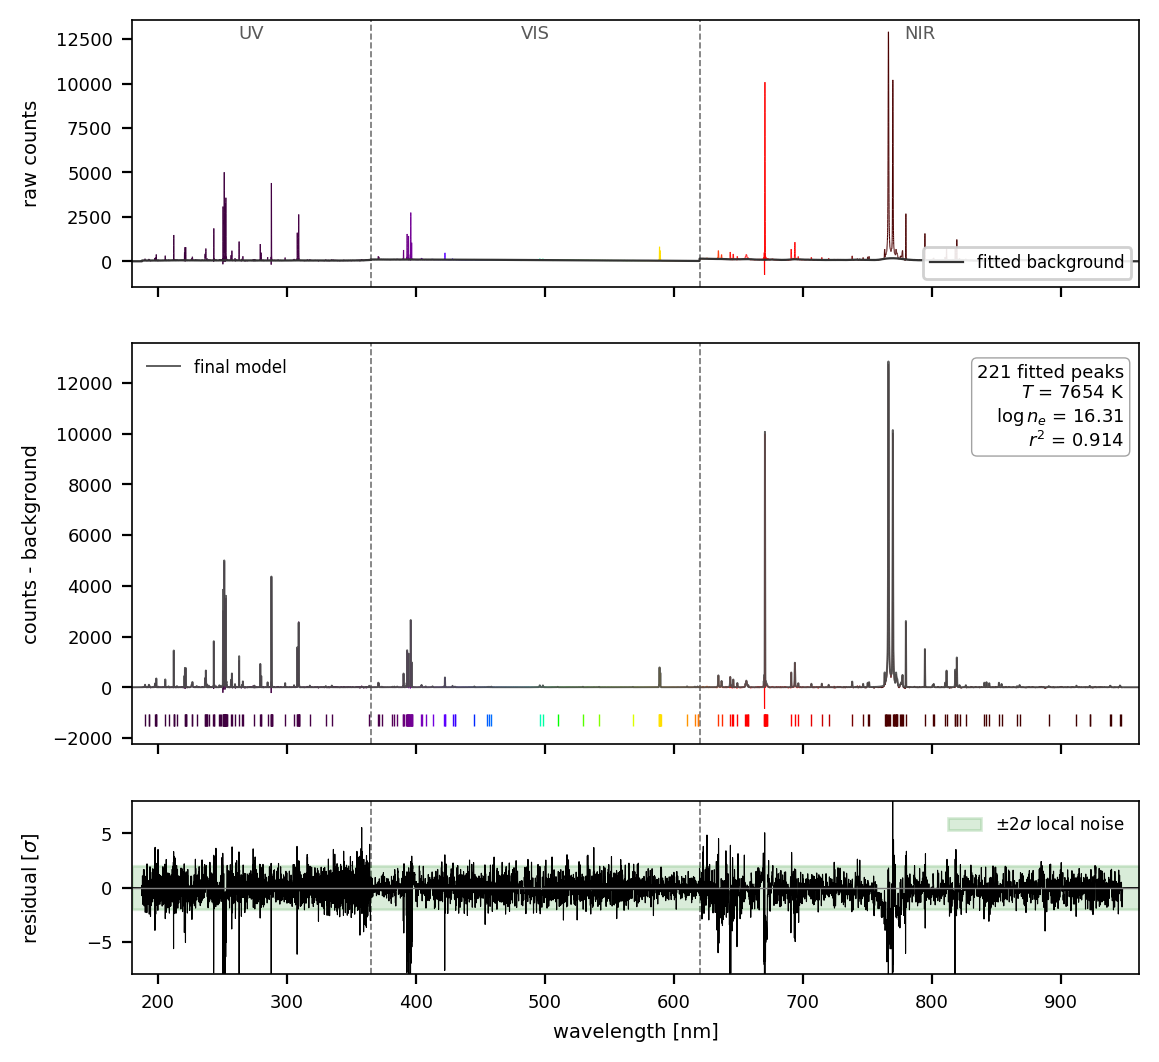
\includegraphics[width=\textwidth]{F1-overview}
\caption{Pipeline overview on the \texttt{user\_spec1} field spectrum. (a)~raw counts with the fitted background; (b)~background-subtracted data with the final model and a wavelength-tinted tick at every fitted peak centre; (c)~residual in units of the local noise $\sigma$ with the $\pm2\sigma$ band. Dashed lines mark the SciAps segment seams at 365 and \SI{620}{\nano\metre} that separate the UV, VIS, and NIR detector segments; the residual structure that exceeds the band is self-absorption, not noise: the largest excursion ($\approx-7\sigma$) is at Li\,I \SI{670.8}{\nano\metre}, with further structure at the Ca\,II H\&K and K\,I 766/\SI{770}{\nano\metre} resonance lines.
The final solve retains 221 fitted peaks and converges to $T=\SI{7654}{\kelvin}$, $\log_{10}(n_e/\mathrm{cm^{-3}})=16.31$, and $r^2=0.914$. % src: manuscript/figures/cache/user_spec1.json
\label{fig:overview}}
\end{figure*}

\subsection{Instrument and data model}
\label{sec:wf-instrument}

The instrument for which the pipeline was developed and validated is a SciAps Z300
handheld LIBS analyzer operated under an argon purge.
Its spectrometer records three CCD segments covering the ultraviolet, visible and
near-infrared, with junctions at \SI{365}{nm} and \SI{620}{nm}.
Each segment has its own wavelength-to-pixel map, so the pixel pitch is not constant:
approximately \SIrange{0.096}{0.079}{nm} per pixel in the ultraviolet segment,
\SIrange{0.142}{0.113}{nm} in the visible, and \SIrange{0.198}{0.156}{nm} in the near
infrared.
A line of a typical width of \SIrange{150}{320}{pm} therefore spans only about
$1.3$--$2.2$ pixels full width at half maximum, at or below the Nyquist limit in the visible
and near infrared.
The junction at \SI{620}{nm} also carries a gain step of roughly a factor of five, which would distort the cross-segment intensity ratios on which Boltzmann and Saha inference relies; it is estimated from the continuum and divided out of amplitudes and uncertainties before every solve (the step at \SI{365}{nm} is additive and is left to background subtraction).

The native record of one acquisition contains 7{,}914 samples.
Of these, 2{,}066 form a fourth, placeholder channel at \SIrange{960}{961}{nm} that carries
no signal and is excluded, leaving 5{,}848 usable samples from \SI{187.8}{nm} to about
\SI{951}{nm}, with a real gap of about \SI{12}{nm} at the red end of the near-infrared
segment that must be masked rather than interpolated.
The vendor's own export resamples the native pixels onto a uniform
\SI{0.0333}{nm} grid with a cubic spline, and an earlier acquisition path used linear
interpolation onto the same grid.
Neither adds information.
In a paired comparison on eight iron runs stored in both forms from the same shots, noise in
the native samples was white (lag-one autocorrelation 0.12), whereas the linearly
interpolated file was strongly correlated (0.76), so a resampled spectrum looks smoother
without being more informative.
\alibz\ therefore processes native pixels.
It accepts any strictly increasing two-column wavelength--intensity file, takes the
pixel pitch from the median grid step, and makes no assumption of a $1/30$~nm grid.
Native fitting required replacing free-width profile fits, which are ill-posed at fewer than
two samples per line width, by estimators that fix the instrument width in pixels
(Sections~\ref{sec:wf-fit} and \ref{sec:wf-registration}).

Two properties of the axis are handled upstream.
Native Z300 spectra initially lacked a pixel offset of $-18$ pixels, so lines appeared \SIrange{1.6}{3.3}{nm} too blue; after the correction a residual of about $-0.25$ pixel remains (Section~\ref{sec:wf-registration}).
The database stores vacuum wavelengths, which the loader converts to the instrument convention (standard air above \SI{200}{nm}, vacuum below) \citep{edlen1966refractive,ciddor1996refractive}; without conversion every line is displaced by \SIrange{0.11}{0.24}{nm}. % src: git 5daafa2 (110-240 pm -> 27 pm median on MW2-112)
Each record analyzed is either a single shot (the MW2-112 scan) or the instrument's own
shot average (ten shots for the Z300 calibration runs); the pipeline treats both as one
spectrum and does not aggregate across records.

\subsection{Background estimation}
\label{sec:wf-background}

The continuum is estimated by asymmetrically reweighted penalized least squares
(arPLS) \citep{baek2015arpls}, a baseline smoother in the family of
Eilers's penalized smoothers \citep{eilers2003smoother}: the baseline minimizes a weighted squared residual plus a
second-difference roughness penalty, and the weight of any pixel above the current
baseline is driven toward zero over successive iterations, so that emission lines of any
width cannot attract the baseline.
Two choices adapt the method to this instrument.
First, the smoothing penalty is set from a \emph{physical} length rather than a number of
pixels: the penalty weight is $(\ell/\Delta\lambda)^4$ for a smoothing length $\ell$ of
\SI{1.9}{nm} and the local pitch $\Delta\lambda$, so the stiffness is the same on all three
segments and on any wavelength grid.
Second, the spectrum is split at the detector junctions and each segment is solved
independently, so that the penalty never spans a hardware step.
On MW2-112 the omission of this split left a $+54$-count ledge at \SI{620}{nm} that
produced spurious peaks; with per-segment solves the ledge was removed.

A failed baseline solve falls back to a zero baseline, and segments are not blended across junctions, so a line straddling \SI{365}{nm} or \SI{620}{nm} is divided between two solves.

\subsection{Peak detection and profile fitting}
\label{sec:wf-fit}

\paragraph{Detection.}
Candidate peaks are strict local maxima: a sample must exceed four of its five window
neighbors.
A maximum is retained only if its intensity exceeds a significance floor of three times
the local noise, and a user-supplied excess is added to, not subtracted from, that floor.
The local noise is a robust point-to-point estimate (the median absolute successive
difference, scaled to a Gaussian standard deviation, evaluated at several lags and taken at
the largest), computed in blocks that restart at each detector junction so that noise from
one segment does not leak into another.
Flat-topped maxima fail the strict test and are recovered by refinement.

\paragraph{Windowed Voigt fits.}
Each detected peak defines a half-maximum window, within which the line is fitted by a
Voigt profile \citep{olivero1977voigt,thompson1987voigt} with parameters
$[A,\lambda_0,\sigma,\gamma]$, where $A$ is the \emph{integrated area}.
This convention is central: the profile is unit-area normalized, so seeding from a
measured height rather than from an area would overestimate the area of narrow lines by
roughly a factor of four.
The fit is bounded: non-negative area, widths limited to a multiple of the median width, center within one sample of its seed.
The modeled contribution of other fitted peaks is subtracted from each window first, so that strong wings do not act as an unmodeled pedestal.

\paragraph{Shoulders and block-coordinate refit.}
Residual structure above two standard deviations of the residual is searched for
unmodeled maxima, and a new component is added wherever one lies farther than one
linewidth from an existing peak, with the existing peaks held fixed.
The components are then refitted jointly, strongest first, in overlapping blocks of
$\pm 50$ samples, the out-of-block components being subtracted as a fixed pedestal.
This is a block-coordinate refit, not a single joint solve over several hundred peaks.
The widths are capped at the window span.
The cap was added after an unbounded fit allowed a single component of
$\sigma = \SI{289}{nm}$ to absorb \SI{89}{\percent} of the fitted area of its window.
Finally, components wider than one hundred times a robust median width
(baseline remnants) are discarded, sub-sample widths are set to zero, and a component
survives only if its implied height exceeds twice the local noise.
On MW2-112 spectrum~0, this first pass returned 303 peaks.

\paragraph{Per-segment peak location.}
Because the lines are barely sampled (Section~\ref{sec:wf-instrument}), the way a line
center is read from the samples matters at the picometer level.
A paired study on 26 iron and 87 vanadium runs on the corrected axis compared a
three-point parabola, a root of the vendor-style cubic spline, a free-width pixel-integrated
Gaussian, and an empirical line-spread function (ePSF) built from the data
\citep{anderson2000epsf}.
No single estimator was best on all segments.
In the visible, the ePSF located iron lines with an error of \SI{5.3}{pm}, against
\SIrange{11.6}{12.3}{pm} for the spline-based estimators.
In the ultraviolet the spline estimators were better (\SIrange{4.7}{4.8}{pm} against \SI{7.6}{pm}), and in the near infrared, tested on argon~I lines because iron lines are absent, a point Gaussian beat the spline (\SI{4.8}{pm} against \SIrange{14}{15}{pm} at \SI{696.54}{nm}); the near-infrared ePSF is withheld because of a location bias at its sub-band seams.
The pipeline therefore dispatches the location method \emph{per segment}, from a packaged
shape file (ePSF in the visible, spline root in the ultraviolet, point Gaussian in the
near infrared), and falls back to the spline root or the Gaussian refinement for any grid
that is not recognized as Z300-native.
The located centers and fit diagnostics are recorded for every refined peak and drive the wavelength registration; the identification stages still consume the blind Voigt centers, pending a dedicated accuracy benchmark.

\subsection{Refinement: blends, phantoms and self-absorption tags}
\label{sec:wf-refinement}

A first-pass fit with symmetric profiles fails in two ways on real spectra.
A self-absorbed, flat-topped line is split into two \emph{phantom} components, and a
genuine blend narrower than one linewidth is fitted as one component.
The refinement stage re-examines every ambiguous feature (sub-linewidth pairs of
components and significant residual structure) under three local models: a single
symmetric Voigt (S), a Voigt attenuated by a cold absorber of the same shape, the
self-absorption profile of Eq.~\eqref{eq:sa-voigt} (A), and two symmetric Voigts (B).
The models are compared by the Bayesian information criterion \citep{schwarz1978bic},
with the raw $\chi^2$ rescaled by the reduced $\chi^2$ of the best model (floored at one),
so that the margin measures relative improvement on windows dominated by systematic
residuals rather than by photon noise.
Fits use a robust soft-$L_1$ loss \citep[cf.][]{huber1964robust} whose scale leaves the five-to-seven-sigma Voigt misfit on the brightest lines un-downweighted, since that misfit is model inadequacy and not outlier contamination.

The verdict is then gated by physics.
A blend is accepted only if the database supplies two \emph{distinct} lines matching the
two fitted centers with a consistent separation, with a BIC margin of 10 (30 without
database support).
An asymmetric verdict is applied only if the primary line has a resonance-capable lower
level ($E_i \le \SI{0.2}{eV}$), the class of lines that self-absorb, and the fitted
emission center has not walked off that line; otherwise it is recorded under a qualified
verdict (nonresonant, displaced or saturated) and left alone.
A fitted optical depth at the fit ceiling is never acted on.

Refinement is staged.
Stage~3a runs before any identification and applies only the data-only actions (blend
splits and single merges), deferring the whole asymmetric family.
Stage~3b runs after pass~1, when a provisional element posterior exists, and adjudicates the
deferred features with the resonance gate conditioned on the \emph{candidate species the
whole-pattern solve retained}, a set broader than the established elements (so that a
wrong pass-1 basin cannot veto a real resonance merge) but far narrower than the periodic
table.
The merge zones are computed before any seeding, and the seeder, residual recovery, deblending and self-absorption recovery all honor them; seeds that landed inside merge zones had eroded the observed areas of merged rows by \SIrange{21}{93}{\percent}.

A merged self-absorbed row carries two areas, and the distinction is important for
quantification.
The \emph{observed area} is the integral of the attenuated profile actually seen, corrected
for the Lorentzian flux outside the fit window.
The \emph{emission area} is the unattenuated, thin-equivalent area of Eq.~\eqref{eq:escape},
proportional to the quantity that enters Eq.~\eqref{eq:emissivity}.
The first version of the merge replaced the fitted components by the narrow absorbed core of the self-absorption model with its wing-inflated area; on MW2-112 spectrum~1000 this overshot the observed core by up to $19\sigma$ at \SI{280.2}{nm}, deleted neighbors that reappeared as $40\sigma$ residuals, and almost doubled the global $\chi^2/\sigma^2$ (32{,}821 after stage~3a to 51{,}701 after 3b).
The verdict is therefore now a \emph{non-destructive tag}: the table keeps the data-faithful symmetric fit, and the emission area and optical depth ride along as metadata for the later growth-curve recovery.
With tags, stage~3b improves the fit (to 28{,}262) and unmodeled residuals above $3\sigma$ fall from 61 to 28.
The symmetric proxy conserves flux but not shape and therefore leaves a core-shaped residual on a flat-topped line, which is a storage choice and not a failure of the model.
On MW2-112 spectrum~0 the residual of the self-absorption model in each merged window was
2--8 times lower than that of the stored symmetric proxy (Li~I \SI{670.7}{nm}, K~I
\SI{766.5}{nm}, Fe at \SI{261.2}{nm}), and the ratio of emission to observed area ranged from 1.24
to 7.0 over fifteen merged lines.
The one genuine cost occurs in crowded windows: where seven components collapse into one (\SI{383.0}{nm}) the model underfits (residual 549 against 76 for the two-phantom fit).
The refinement reduced the first-pass fit from 303 to 288 peaks.

Two further profile-level actions run after the identification passes, each gated and
excluded from merge zones.
\emph{Shoulder deblending} refits a peak whose residual shows a one-sided flank bump as two
components plus a pedestal, the main component confined near its parameters and the new
one pinned at the bump, accepted at a matched-filter signal-to-noise ratio of 4 and a window
BIC margin of 6.
\emph{Self-absorption area recovery} (Section~\ref{sec:wf-solve}) refits sa-like peaks
of species that are not already doublet-anchored.
On the 38 JChristensen drill-core spectra, deblends fired on 26 and recovery on 24.
Figure~\ref{fig:refinement} shows the two resonance-line decisions on MW2-112 spectrum~1000.

\begin{figure*}[t]
\centering
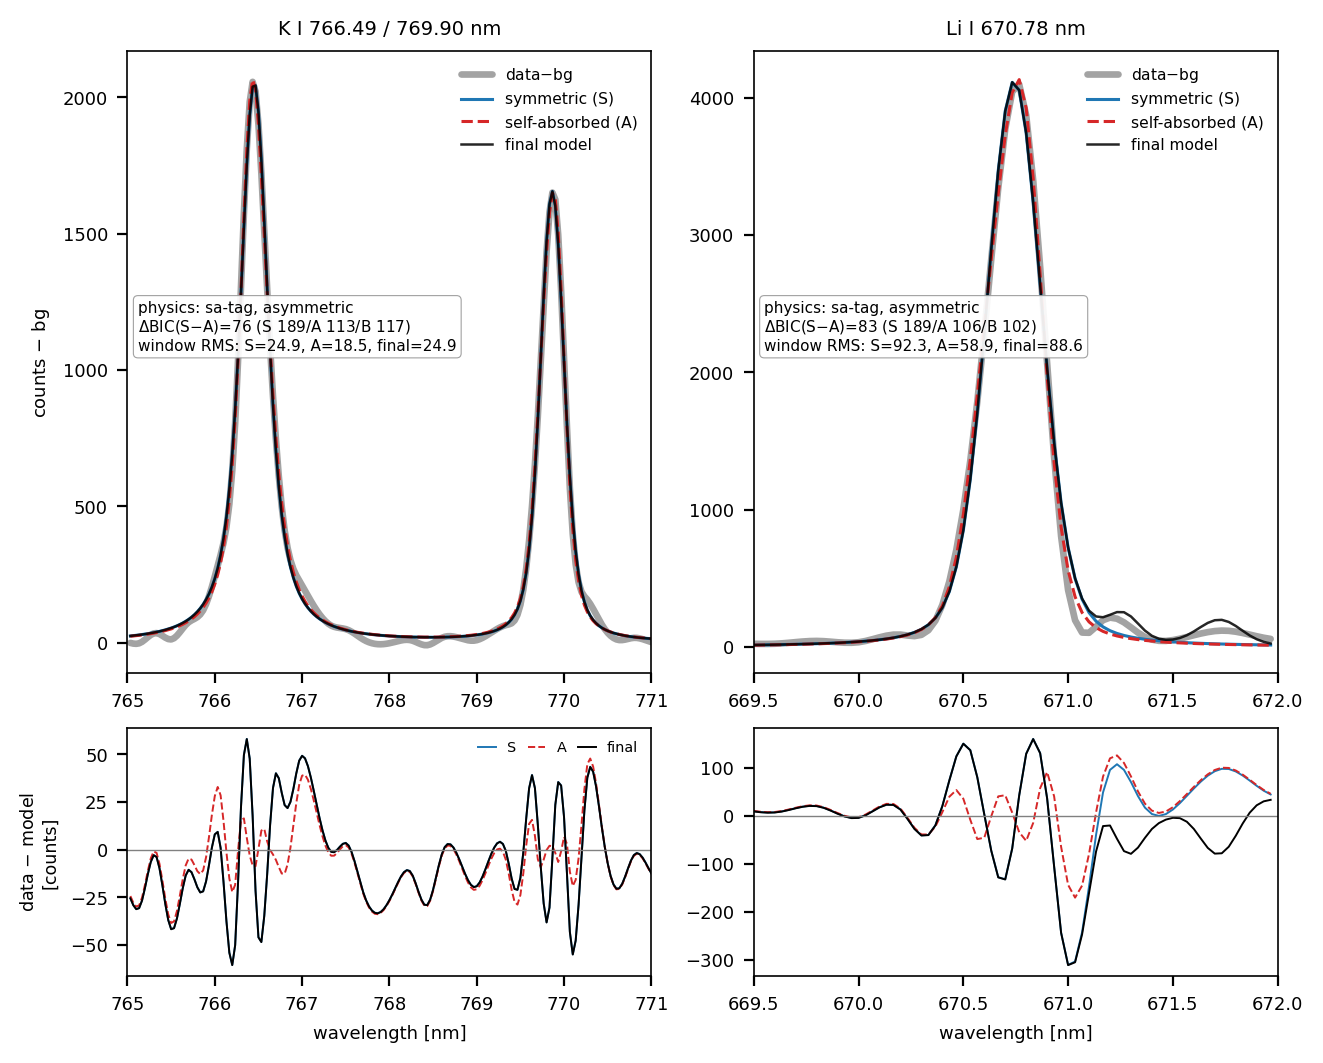
\includegraphics[width=\textwidth]{F3-refinement}
\caption{Self-absorption refinement in two resonance windows of MW2-112 spectrum~1000 (the K window spans both the 766.49 and \SI{769.90}{\nano\metre} doublet lines): the symmetric single Voigt (S), the self-absorbed profile of Eq.~\eqref{eq:sa-voigt} (A), the final model, and the three residuals below. On this spectrum both lines are resolved as non-destructive self-absorption \emph{tags} (verdict asymmetric), not as the phantom-split merge seen on spectrum~0: the tag keeps the data-faithful symmetric envelope in the model (so the final residual tracks S) while recording the attenuated-emission metadata, and the A profile that fits the reversed core more closely is the statistically preferred shape.
K\,I \SI{766.49}{\nano\metre} gives $\Delta\mathrm{BIC}(S{-}A)=76$ with in-window residual RMS of 24.9 (S), 18.5 (A), and 24.9 counts (final); Li\,I \SI{670.78}{\nano\metre} gives $\Delta\mathrm{BIC}=83$ and RMS 92.3, 58.9, and 88.6. % src: manuscript/figures/cache/mw2_1000.json
\label{fig:refinement}}
\end{figure*}

\subsection{Wavelength registration}
\label{sec:wf-registration}

Matching a peak table against a database requires an axis registered to a few tens of picometers, so registration is measured on each spectrum.
The most trusted references are the Ar~I and O~I lines that are present because of the
argon purge and the ambient air; they are independent of the sample and lie almost
entirely in the near-infrared segment.
Their set of anchors (696.5, 706.7, 738.4, 750.4, 763.5, 772.4, 794.8, 801.5, 811.5, 826.5,
842.5 and \SI{912.3}{nm}) registers as genuine argon to within about $\pm\SI{30}{pm}$ on
the corrected axis, with ten to twelve clean lines per run, so that the near-infrared segment
passes its three-line gate on essentially all runs.
Second, a deterministic estimator measures \emph{golden lines} of the declared composition,
selected as lines in the segment's strongest predicted set with no composition, argon,
nitrogen, oxygen or hydrogen line of non-negligible strength within $\pm\SI{0.5}{nm}$,
centered by the point-Gaussian fit and combined by a Huber estimate into a per-segment
offset; fewer than three golden lines leave the segment unregistered.
A vote-mode estimator is retained as a diagnostic only. Only the \emph{offset} is applied; the fitted slope is a diagnostic, because the strongest near-infrared metal lines are optically thick and displaced.

The measured behavior justifies this restraint.
On the corrected axis the residual calibration error is about $-0.25$ pixel in the
near-infrared segment (median $-0.25$ pixel from an Ar~I cross-correlation recorded with each run, $-0.26$ pixel
from the ambient Ar~I shift, 107 runs), but it is \emph{not} a constant: it is $\approx 0$
for one calibration epoch, $\approx -0.28$ pixel for another, and swings from $-0.5$ to $+0.25$
pixel from run to run.
It is therefore a per-calibration residual to be measured on each spectrum, not a fixed
offset.
The per-segment offset transfers between metals (iron to vanadium in the visible: \SI{40}{pm} against \SI{597}{pm} on the uncorrected axis), with a run-to-run standard deviation of at most \SI{12}{pm} in the visible.

The default mode applies the composition-independent ambient registration to the near-infrared segment and keeps the legacy mixed-element anchor shift elsewhere. The element registration is recorded but not applied by default, because changing the inversion's wavelength input pipeline-wide should be gated on an accuracy benchmark.
A second argon-based engine (regional Ar~I and O~I offsets, applied only inside its bracketed anchor support when at least three consistent groups agree) runs alongside; the two argon estimates are cross-checked and a flag is raised beyond three standard errors.
All shifts follow the convention observed $-$ database.

The mixed-element legacy shift is also estimated \emph{per segment}, from the
\emph{refined} table, and a segment's own median is adopted only when it
has at least five unambiguous matches and deviates from the pooled global median by more
than twice the median's standard error.
The gate is essential.
On MW2-112 the per-segment medians differed by \SIrange{10}{35}{pm} but with
median absolute deviations of \SIrange{26}{71}{pm}, so the gate refused and behavior reduced to
the global shift; when the gate was removed, a $+\SI{20}{pm}$ pseudo-shift in one segment
conjured \SI{25}{\percent} phantom Ti in MW2-112 spectrum~1000.

\subsection{Prior-driven minor-line seeding and iterative deepening}
\label{sec:wf-seeding}

Once an element is established from its strong lines, the remaining lines of that element
in the same ion stage are predicted: within one stage, Eq.~\eqref{eq:emissivity} fixes all
line ratios up to a single per-(element, stage) scale, which is measured from the
stage's clean strong lines.
The seeding stage uses those predictions to fit lines the blind pass rejected, and to
deblend an established line hidden beneath a stronger line of another element.
Scale calibration admits a database line as a reference only if its same-element multiplet
contamination is at most \SI{10}{\percent}, its nearest fitted peak lies within \SI{0.06}{nm} and
clears a noise-derived amplitude, and no other peak blends it; the scale is the robust
median of area over predicted strength, and its spread is the median absolute deviation.
A stage predicts only when at least three consistent references exist and the spread is
bounded.
A stage is \emph{falsified} if its brightest predicted line would far exceed anything matched
(the case of a spurious Na~II), and every addition must agree with its Boltzmann prediction
to within a factor of five, or it is recorded as inconsistent or missing and not added.
Importantly, the acceptance decision is made on a prior-\emph{free} area, a non-negative
least-squares area against a frozen-geometry basis \citep{lawson1995nnls}, together with a
BIC improvement: the prior justifies looking for a line, but the data decide whether it is
there.
The module assumes a single reference temperature of \SI{0.76}{eV} ($\approx\SI{8.8}{kK}$,
the corpus median for MW2-112) and optically thin emission, and does not couple ion stages
(the Saha coupling of Eq.~\eqref{eq:saha} belongs to the solve).
On MW2-112 spectrum~0 the first-pass fit of 303 peaks became 288 after refinement and 299
after seeding.

Seeding as a single pass was replaced by \emph{iterative deepening}.
The earlier design seeded once and then re-optimized the plasma state (pass~3), which on drill-core data drifted into a low-temperature basin ($\approx\SI{5200}{K}$) where one line-rich element explained everything while $r^2$ improved.
In the current design, the ions that are \emph{quantified from their intense peaks}, those
with at least four clean reference lines in some stage, have earned a lower
recovery bar for their own faint lines.
In each round, at a successively lower local-noise bar (currently $3.0\sigma$ and then $2.0\sigma$),
these ions are seeded from the Boltzmann prior and, in addition, residual peaks are
recovered from the data without a prior, but only where a confident ion's own database line
marks the position; empty regions keep the full $4\sigma$ bar and cannot admit chance
coincidences.
The composition is re-solved at the \emph{fixed} pass-2 plasma state, so that the weak lines
corroborate and cannot move the temperature; the re-solve reproduced the optimizer's final
solve to machine precision on its own state, and a round is rejected wholesale if it newly
collapses the composition (Section~\ref{sec:wf-solve}).
On MW2-112 spectrum~1000, deepening added 41 lines (23 seeded and 18 recovered) in three
rounds, under an earlier three-bar schedule, without collapse, in about \SI{264}{s} end to end.

\subsection{Whole-pattern solve}
\label{sec:wf-solve}

\paragraph{Candidates and design matrix.}
The solver is run twice, as pass~1 (provisional) and pass~2 (warm-started at the pass-1
state).
For a trial plasma state, every database line of every candidate element and ion stage
contributes a column of the Saha--Boltzmann design matrix (Eqs.~\eqref{eq:emissivity} and
\eqref{eq:saha}), and the observed peak areas are modeled as the non-negative combination
of columns that minimizes the amplitude misfit.
Candidates are pruned by an evidence prefilter, and a provisional pass-1 rejection cannot
prohibit later recovery, because passes~2 and deepening rebuild their candidates from their
own peaks.
The default objective is the non-negative least-squares fit; the weighted variant
(Eqs.~\eqref{eq:wnnls} and \eqref{eq:sigma-eff}) is implemented but is an opt-in, since in
tests on synthetic Ca--Mg scenes it was accurate at the true plasma state but its $\chi^2$
still misranked the temperature; it stays off until that bias is resolved on the synthetic suite.
When the weighted solve is used, the additive amplitude floor of Eq.~\eqref{eq:sigma-eff} is
set from the spectrum's own noise scale, because the sigma from the fit collapses where
the local window is quiet.

\paragraph{Plasma state.}
Temperature and electron density are found by a search over $(T,\log_{10}\nel)$.
The default search evaluates a $15\times 7$ grid of profile objectives and seeds a
Gaussian-process optimizer \citep{jones1998ego} from it; the grid became the default because
the objective has a narrow valley along the Saha $(T,\nel)$ ridge, which the
cold-started optimizer missed on every spectrum tested, and the grid seeds land on the ridge.
The amplitude objective is flat in $\nel$ at fixed temperature, so $\nel$ is set by a prior:
the Stark width of H$_\alpha$ \citep{gigosos2003halpha} when present, and otherwise a default of
$\log_{10}\nel = 17.0 \pm 0.5$ (in cm$^{-3}$) with the search restricted to
$\pm 1\sigma$ of it.
The restriction costs no data fidelity, since the objective is flat in $\nel$, and
it prevents the stage-consistency thermometer, which sees $\nel$ only through the Saha
degeneracy, from sliding to the cold end of the ridge.
In the synthetic Ca--Mg tests this box gave Ca/Mg $=0.52/0.48$ at \SI{8.9}{kK} (truth $0.6/0.4$ at
\SI{10}{kK}), whereas a $2\sigma$ box gave \SI{8.2}{kK} and a wrong order.
A result at the edge of the box is flagged.
The cost includes the stage-consistency term of Eq.~\eqref{eq:tie-cost}, weighted at unity,
so that the Saha--Boltzmann stage ratio is trusted exactly as much as the observed amplitudes;
setting the weight to zero recovers the historical thermometer based on within-stage
Boltzmann ratios only.

\paragraph{Collapse guard.}
On drill-core spectra the single-element dominance failures (Hg at 1.000, Fe at 0.991,
Ca at 0.990) were \emph{not} peak-shape failures: the driver peaks classified as
instrumental.
They were inverse-solve basin failures, in which a corroboration re-index drifted to a
low-temperature basin where one element's tiny response explained everything while
$r^2$ \emph{improved} (to 0.87), because a line-rich element can fit anything.
A corroborated composition is therefore rejected when its top fraction reaches
\SI{90}{\percent} and has grown by at least $0.2$ over the pass-2 top fraction; the summary records
\texttt{corroboration-rejected(collapse)}.
In A/B tests Hg 1.000 became K, Li and Si, and Fe 0.991 became Si, K and Li.
The guard complements shape quality control, which flags abundances resting on saturated or overlap-contaminated peaks; goodness of fit alone cannot compare basins.

\paragraph{Detectability gate.}
An element is dropped if its strongest predicted line does not clear $z_{\min}=3$ times the
local \emph{area} noise of the peak, a statistic (Eq.~\eqref{eq:detect}) that is immune to a
single dominant line and admits arbitrarily many low-concentration elements provided each
shows one real line above noise.
Without a noise model (a bare indexer) only a zero-column activity test applies, so the gate
cannot over-exclude in code paths lacking one.
On MW2-112 spectrum~1000, Bi, which pass~1 had assigned a fraction of 0.94 on the strength of an
ill-conditioned estimate whose predicted strongest line was four counts, had $z = 2.2$,
against $z \ge 4.6$ for every real element (Mn 4.6, Be 6.8, up to K at 103); the gate also
removed an Hg phantom (0.27, $z=0.5$) and left a silicate assemblage of Si 0.75, Fe 0.09,
Al 0.05 and Ti 0.04 together with the real Be, Rb, Na and Ca traces.

\paragraph{Confounder contest and resolution.}
For every detected element, the contest of Eq.~\eqref{eq:contest} asks whether a rival could
cover the element's supporting peaks without violating its own true negatives, scanning a
corpus-plausible plasma grid ($T\in\{6,8,10,12\}$~kK, $\log_{10}\nel\in\{16.5,17.5\}$)
against a pre-prune candidate table built at \SI{9}{kK}, because a wrong attribution drags
the fitted state to where the rival's lines vanish and the error then certifies itself.
A supporting peak is contested if a rival, at the largest concentration its own true
negatives allow, still covers at least half of the peak's amplitude, using the rival's
non-resonance lines to set that cap so that self-absorbed resonance lines do not
understate it.
An element whose every supporting peak is contested is demoted to \emph{confounded}.
On the drill-core spectra, two hot-Mn results (40--53\,\% Mn, resting on two peaks inside
the Mg~II 279.553/\SI{280.270}{nm} doublet region) were demoted with a contested share of 1.0
and the confounder Mg, while independent Li, Al and Na detections were untouched.
The reported composition then credits a confounded element only its clear flux and
reattributes the contested remainder to the confounder, under two guards: the response
ratio is clamped at one, and a rival receives flux only up to its own evidence ceiling
(zero if the fit pruned it).
Without the first guard a 3.8\,\% Be confound became a 42\,\% Fe phantom.
The result is Mn $53\%\to 0\%$ and Mg $8\%\to 31\%$.

\paragraph{Self-absorption recovery re-solve.}
For sa-like peaks of species not anchored by a resolved doublet, the self-absorption model
is refit against a symmetric control, accepted only with a BIC win of 10, an optical depth
below the ceiling, and an amplification of at most five.
Accepted emission areas replace the observed amplitudes, and the composition is
\emph{re-solved linearly} at the fitted plasma state, with no new Bayesian pass and no basin
risk, and the collapse guard is applied to the corrected composition as a final safeguard.
Doublet-anchored species (K~I, Na~D) are skipped, since their depths already act on the response side and correcting the data side too would double-count.
The pre-measured emission-to-observed ratios of merged lines are propagated through the same re-solve.
On the JChristensen set, corpus means moved by $+3.1$ percentage points (Si) and $-3.5$ (K) with no collapse; on MW2-112 the recovered lines (Al~I \SI{396.1}{nm}, Mg~I \SI{383.8}{nm}) carried optical depths near $0.5$.

\paragraph{Uncertainties.}
Statistical uncertainties on the fractions come from resampling the peak amplitudes within
their uncertainties (32 draws by default) and re-solving at the fitted state
\citep[cf.][]{efron1979bootstrap}.
They do not include the systematic error of the LTE assumption, of the atomic data, of matrix
effects or of unresolved self-absorption, and the reported fractions should be read
accordingly.

Figure~\ref{fig:walkthrough} follows MW2-112 spectrum~1000 through the stages and across the successive solves.

\begin{figure*}[t]
\centering
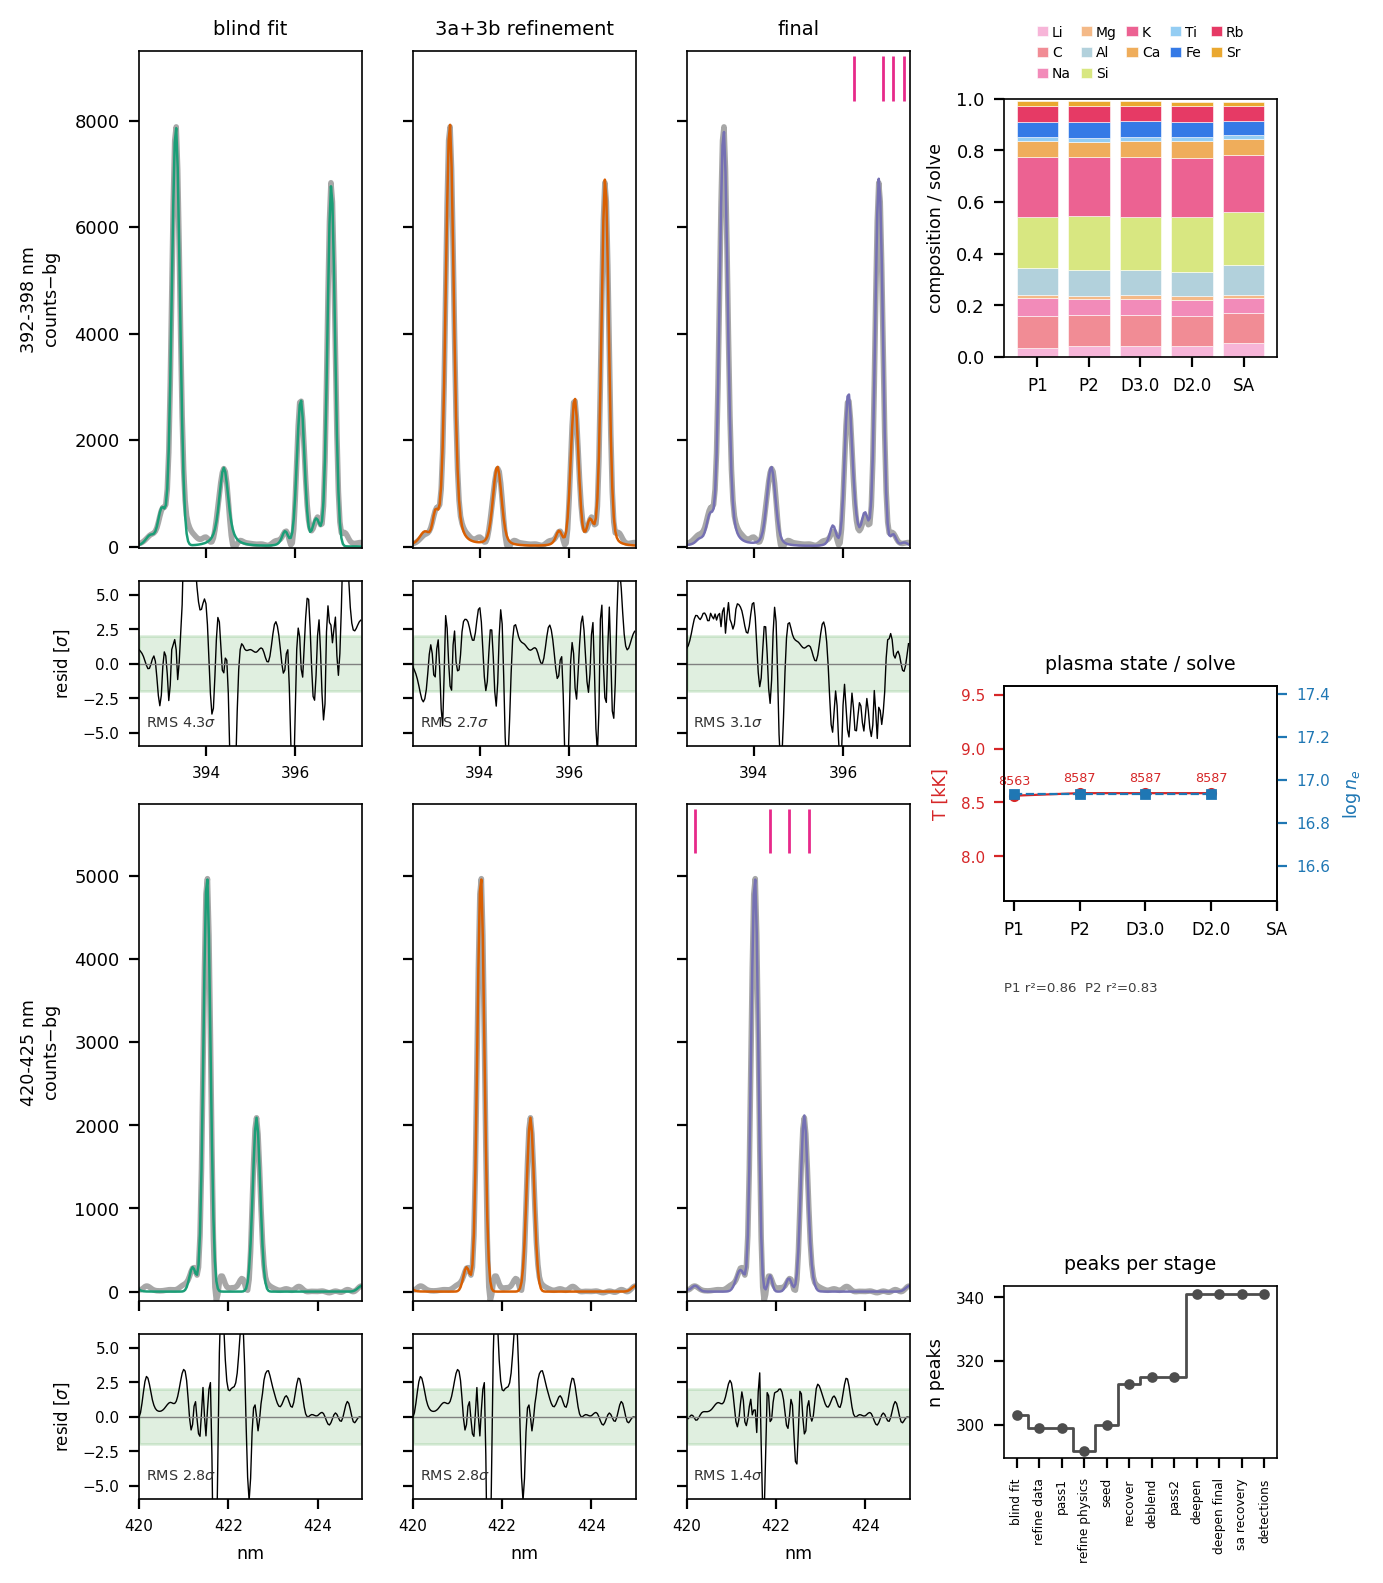
\includegraphics[width=\textwidth]{F2-walkthrough}
\caption{Stage-by-stage walkthrough of MW2-112 spectrum~1000. Left: two windows chosen for visible stage change (a Ca-rich window at \SIrange{392.5}{397.5}{\nano\metre} and a line-dense window at \SIrange{420}{425}{\nano\metre}), each shown after the blind fit, after data and physics refinement (3a+3b), and at the final model; the thick grey trace is the data, the coloured line the stage model, pink ticks mark peaks new to that column, and each residual strip (local-$\sigma$ units) carries its per-column RMS. Right: composition of every element with final fraction $\ge0.01$ across the pass-1, pass-2, accepted deepening, and self-absorption-recovery solves, the plasma state (T annotated, $r^2$ per solve), and the peak count per stage.
The peak count grows from 303 (blind) to 341 (final); the temperature moves only from \SI{8563}{\kelvin} (pass~1) to \SI{8587}{\kelvin} (pass~2) at fixed $\log_{10}(n_e/\mathrm{cm^{-3}})=16.94$, and the largest change of any element fraction across the five solves is 0.019 (Al), so the composition is stable once established; the final solve is led by K~0.22, Si~0.20, Al~0.12, and C~0.11 at $r^2=0.62$. % src: manuscript/figures/cache/mw2_1000.json
\label{fig:walkthrough}}
\end{figure*}

\subsection{Outputs}
\label{sec:wf-outputs}

The command-line entry point runs the chain over a directory of spectra in parallel workers and writes four products.
\texttt{summary.csv} has one row per spectrum: plasma parameters, detected-element fractions with statistical uncertainties, and diagnostic flags (goodness of fit, electron density at the search bound, stage disagreement, confounded and dominant-weak-shape elements, collapse rejection).
\texttt{detections.csv} is in long format, one row per sample and element: status, line support, $z$-scores, upper limits, clear-line and contested-share accounting, and the as-fit and resolved fractions.
\texttt{background\_gases.json} and \texttt{wavelength\_calibration.json} record the Ar~I and O~I evidence and the independent wavelength references, with the regions in which any correction was applied.
An inspection notebook (\texttt{fit\_inspection.ipynb}) shows the fits, refinement decisions, seeded lines and composition for one spectrum.
Unless disabled, a run manifest records the git state, configuration snapshot and input hashes, so that a reported number can be traced to the code and configuration that produced it.
The partition-function cache reduced the run time for a median spectrum of 410 peaks from
\SI{225}{s} to \SI{106}{s}. % src: git e715ff0 (MW2-112 id1518, 2.1x end to end)

\section{Datasets}
\label{sec:datasets}

The validation strategy of this work is a ladder of increasing realism and decreasing certainty about ground truth (Section~\ref{sec:results}): synthetic spectra for which every plasma parameter is known by construction; real spectra of a lithium-bearing mudrock and of drill-core samples for which no assay is held in the repository; and pure-element standards measured on a handheld LIBS analyzer, for which the composition is known but the matrix is far from geological. Table~\ref{tab:datasets} lists every dataset used, its role, and what, if anything, constitutes ground truth. Throughout, ``repository'' means the \alibz{} source tree; several datasets are too large to be committed and are identified by a pointer instead.

\begin{table*}[t]
\centering
\footnotesize
\setlength{\tabcolsep}{3pt}
\caption{Datasets used in this work. ``Role'' is development (used to tune or debug the pipeline), validation (held out from tuning), or calibration (used to estimate instrument properties). Ground truth ``none'' means that no assay or certified composition is available; vendor composition summaries, where they exist, are treated as uncalibrated comparisons only. Paths are relative to the repository root.}
\label{tab:datasets}
\begin{tabular}{@{}p{1.05cm}p{2.7cm}p{1.3cm}p{2.3cm}p{1.7cm}p{2.6cm}p{3.2cm}@{}}
\toprule
Name & Instrument and grid & $n$ spectra & Target & Role & Ground truth & Repository location \\
\midrule
Suite S & \alibz{} explicit-stage generator, native Z300-like grid (per-segment pitch) & 5 named cases, seeded & Ca/Mg binary; Si--Ca--Fe--Mg; Si--Al--K--Na; Fe--Ti--Ca; Ca/Mg in argon ambient & Development; regression gate & By construction: composition, $T$, $\log_{10}\nel$, seed % src: bench/synth_cases.py (CASES), alibz/synthetic.py (render default ChannelGrid.native)
 & \texttt{bench/\allowbreak synth\_\allowbreak cases.py}; \texttt{tests/\allowbreak test\_\allowbreak roundtrip\_\allowbreak synthetic.py} \\
NIST-backed benchmark & NIST-line forward model; \SIrange{370}{600}{\nano\metre} at \SI{0.02}{\nano\metre} (defaults) & 3 cases per default run & Random 3--7 element sparse mixtures; $T$ drawn in 7--\SI{13}{\kilo\kelvin}, $\log_{10}\nel$ in 16--17.3 % src: bench/benchmark.py (sample_composition, sample_theta, run_benchmark defaults)
 & Engine comparison & By construction: $T$, $\nel$, composition & \texttt{bench/\allowbreak benchmark.py}; \texttt{bench/\allowbreak nist\_\allowbreak forward.py} \\
MW2-112 & Vendor export, 23\,431 points, 180--\SI{961}{\nano\metre}, $1/30$\,\si{\nano\metre} % src: docs/mw2_112/provenance.md (Raw observations)
 & 929 single-pulse shots, IDs 989--1917 % src: docs/mw2_112/provenance.md
 & Finely stratified lithium mudrock, \SI{100}{\micro\metre} step profile & Development and production-gate case & None; 927 vendor summaries as uncalibrated comparison % src: docs/mw2_112/analysis_plan.md (Input audit)
 & \texttt{docs/\allowbreak mw2\_\allowbreak 112/\allowbreak }; raw spectra outside repository \\
JChristensen & Vendor export, same 23\,431-point grid % src: docs/transformer_plan.md (MW2-112 and JChristensen exports each contain 23,431 rows)
 & 38 % src: docs/development_guide.md (Measured on JChristensen (38 spectra))
 & Drill-core samples (MDD series) & Development (confounders, basin collapse) & None in repository & Raw spectra outside repository; default path in \texttt{scripts/\allowbreak fit\_\allowbreak inspector.py} \\
Remote samples & Vendor export, 23\,431 points % src: data/remote_samples/*.csv (23432 lines each incl. header)
 & 5 & REE\_01, REE\_44, scan9x9, user\_spec1, argon\_noAr & Native-grid recovery; thermometer behavior & None & \texttt{data/\allowbreak remote\_\allowbreak samples/\allowbreak } (local, not under version control) \\
Z300 corpus & SciAps Z300 AverageSpectrum exports & 4\,909 surveyed; 435 with strong continuum % src: corrections/detector.json (segment_response_fallback.provenance)
 & Mixed geological and reference samples & Calibration (620~nm response step, noise statistics) & None & Raw spectra on a lab file server, not in repository; summary in \texttt{corrections/\allowbreak detector.json} \\
Archive survey & Vendor exports of several grid formats & 8\,213 spectra % src: reports/2026-09-20-alibz-review.md (Moissanite archive runs)
 & Archive of earlier campaigns & Native-grid recovery statistics & None & \texttt{reports/\allowbreak 2026-09-20-alibz-review.md} \\
Whole-rock prior & Compilation tables & 1\,022\,092 samples reported % src: docs/whole_rock_prior.md
 & Global whole-rock geochemistry & Scene prior for synthetic training data & Literature compilation & \texttt{db/\allowbreak whole\_\allowbreak rock\_\allowbreak prior\_\allowbreak v1.npz}; manifest in \texttt{db/\allowbreak } \\
Fe standard & Z300-0915, native grid, 5\,848 points, 187.8--\SI{950.7}{\nano\metre} % src: cal/reports/2026-09-24-fe-calibration-plasma-analysis.md (Data)
 & 26 runs, 252 shots % src: cal/reports/2026-09-24-fe-calibration-plasma-analysis.md (Data)
 & Fe, Aesar 99.98\% % src: cal/README.md (Studies)
 & Calibration and validation of line physics & Nominal purity & \texttt{cal/\allowbreak reports/\allowbreak }, \texttt{cal/\allowbreak scripts/\allowbreak }; shots on lab server \\
V standard & Z300-0915, native grid & Run~2: 59 batches in a $5\times4$ delay--period grid, 3 replicates % src: cal/reports/2026-09-24-vanadium-timing-study.md (header)
 & Pure V metal & Calibration (timing, self-absorption) & Pure element, purity not recorded in repository & \texttt{cal/\allowbreak reports/\allowbreak }, \texttt{cal/\allowbreak data/\allowbreak }; shots on lab server \\
\bottomrule
\end{tabular}
\end{table*}

\subsection{Synthetic data}

Two generators provide synthetic ground truth, and they serve different purposes. The first is the explicit-stage generator of \alibz{} itself (module \texttt{alibz.synthetic}), which takes ion-stage abundances directly and applies no Saha balance. Because the inverse model assumes Saha equilibrium, a round trip through it with arbitrary stage abundances would carry model mismatch unrelated to the engine under test. Suite~S (\texttt{bench.synth\_cases}) therefore first converts element fractions into stage fractions through the Saha equation at the scene's $(T,\nel)$ and then renders the scene. Its five frozen cases are a Ca/Mg binary, a four-element silicate-like mixture, an alkali-bearing feldspar-like mixture that exercises the K/Na resonance self-absorption degeneracy, an iron-rich low-temperature mixture, and the binary rendered in an argon ambient. Case names are stable because the scoreboard history is keyed on them; each case is replayable from its composition, $T$, $\log_{10}\nel$, and seed. Rendering scales are matched to SciAps exports (bright lines in the $10^3$--$10^4$ count range, near-zero vendor-subtracted pedestal) % src: bench/synth_cases.py (DEFAULT_EMISSION_SCALE comment)
.

The second generator, in \texttt{bench.benchmark}, draws random sparse compositions and plasma parameters from the NIST-backed forward model of \texttt{bench.nist\_forward} and is used to score two inverse engines on identical data. It was built for a head-to-head comparison in which one engine is handed the candidate element set and the other must discover elements from the full 92-element database; the scorer therefore reports false positives as well as true-element recovery. The prototype engine that this benchmark compared against has since been removed from the source tree, and case generation in the harness still depends on that prototype, so the harness cannot currently be run as written (Section~\ref{sec:results}).

Synthetic training data for the planned learned model are drawn from a natural-composition scene prior fitted to the global whole-rock compilation of Gard et al.~\cite{gard2019wholerock}. The paper reports 1\,022\,092 samples, whereas the pinned release tables contain 1\,023\,490 sample rows; both counts are recorded in the repository rather than reconciled % src: docs/whole_rock_prior.md
. The compilation is heterogeneous and dominated by igneous rocks, so the prior encodes plausible, not representative, compositions.

\subsection{Real geological spectra}

MW2-112 is a finely stratified lithium mudrock profiled at a \SI{100}{\micro\metre} step with a laser spot of approximately \SI{50}{\micro\metre} % src: docs/mw2_112/provenance.md; docs/mw2_112/analysis_plan.md (G1)
. The 929 spectra are consecutive single pulses (IDs 989--1917, with no within-position replicates), exported on the vendor grid of 23\,431 points; the active range is 190--\SI{910}{\nano\metre}. One spectrum (ID 1632) is identically zero and is retained in the inventory as a failed observation rather than as zero abundance, and two acquisition breaks (four and 176 minutes) are recorded % src: docs/mw2_112/analysis_plan.md (Input audit)
. The vendor composition summaries cover 927 of the 929 spectra and are used only as an uncalibrated comparison. Gate delay, gate width, atmosphere, and pulse energy are not recorded in the exports % src: docs/mw2_112/analysis_plan.md (G1)
. The principal product of that campaign is therefore a within-element relative profile, not a bulk composition.

The JChristensen set comprises 38 spectra from drill-core samples on the same export grid. It served as the development ground for two of the failure modes in Section~\ref{sec:results} (confounded attribution of Mn and Mg, and single-element basin collapse) because both were first observed there. Neither dataset has an assay in the repository; for both, correctness is judged by internal consistency, by synthetic round trips that reproduce the failure, and by within-element agreement with independent vendor summaries.

The five files in \texttt{data/remote\_samples} (REE\_01, REE\_44, scan9x9, user\_spec1, and argon\_noAr) are retained locally as small test cases of real vendor exports; the directory is excluded from version control (\texttt{.gitignore} rule \texttt{data/}), so they are identified by name and checksum rather than committed % src: .gitignore line 30; manuscript/data/showcase.json (user\_spec1 sha256)
. They were used to develop native-grid recovery and to compare the pipeline before and after the stage-consistency thermometer; none has a reference composition % src: reports/2026-09-21-stage-consistency-thermometer.md (What remains unverified)
. A larger corpus of Z300 \texttt{AverageSpectrum} files, of which 4\,909 were surveyed, supplied the empirical VIS-to-NIR throughput step at \SI{620}{\nano\metre} used as a fallback response when a spectrum's own continuum is too weak to measure it (median 3.9, interquartile range 3.0--5.2, from 435 spectra with adequate continuum) % src: corrections/detector.json (segment_response_fallback.provenance)
. A separate survey of 8\,213 archive spectra characterized the vendor export formats (97.9\% on the standard $1/30$\,\si{\nano\metre} grid) % src: reports/2026-09-20-alibz-review.md (Moissanite archive runs)
.

\subsection{Pure-element standards on the Z300}

The calibration campaign measured high-purity elemental metals one at a time on a SciAps Z300 (unit Z300-0915) % src: docs/z300_device_notes.md (sec. 1)
, using the native detector grid with no resampling. The iron study comprises 26 runs and 252 shots on Aesar 99.98\% Fe, acquired with argon pre-flush and gated detection, partly on a single reused site (to follow crater depth) and partly on fresh raster sites % src: cal/reports/2026-09-24-fe-calibration-plasma-analysis.md (Data)
. The vanadium studies comprise a first replicated delay/period grid and a second $5\times4$ grid with three replicates; the second suffers from a design confound (one raster lap per delay value, so that delay and crater depth are aliased), which is documented and which limits the conclusions that can be drawn from it % src: cal/reports/2026-09-24-vanadium-timing-study.md (design confound)
. These datasets are the only ones in this work with a known composition measured on the target instrument, but a pure metal is a severe test of line physics (dense line forests, optically thick resonance lines) and a weak test of matrix handling.

All Z300 native spectra used here were re-derived after the discovery that the pixel-to-wavelength map had omitted a fixed offset of 18 detector pixels, which had labeled every line about 1.6--\SI{3.3}{\nano\metre} too blue % src: reports/2026-09-23-native-axis-18px-offset.md
. Results obtained before the correction (reports dated 2026-09-22 and 2026-09-23) are superseded, and only the corrected-axis analyses are used below.

\subsection{Datasets not yet available}

No certified reference materials have yet been measured, so no result in this work is an accuracy statement against a certified composition. Likewise, the planned argon-versus-air composition-invariance test has so far been exercised only on synthetic scenes (the argon-ambient case of Suite~S); the acquisition of a dedicated argon-rich series on a non-argon-bearing target is recorded as a prerequisite for a multi-line near-infrared registration % src: DECISIONS.md (2026-09-23 Two argon wavelength engines, item d)
.

\section{Fit metrics and acceptance gates}
\label{sec:metrics}

A central lesson of the development of \alibz{} is that no single goodness-of-fit number can be trusted to select the right physical solution. This section defines each metric precisely, states where it is computed, and separates metrics that are \emph{reported} from those used to \emph{decide}. Table~\ref{tab:metrics} summarizes them. The equations referred to are those of Sections~\ref{sec:theory} and~\ref{sec:workflow}.

\subsection{Goodness of fit and model comparison}

\paragraph{Residual $r^2$.}
The pipeline reports the coefficient of determination of the fitted peak-amplitude vector against the observed one. It is a quality-control quantity only: it is mapped to a warning below 0.50 and a failure below 0.30 % src: alibz/pipeline.py (FIT_R2_WARN, FIT_R2_FAIL)
. It cannot compare solutions because a line-rich element fits almost any peak list. In a measured basin-collapse failure on the JChristensen set the pass that collapsed onto one element at about \SI{5200}{\kelvin} had an $r^2$ that \emph{improved} to 0.87 % src: docs/development_guide.md (honest measured caveat from JChristensen)
. Likewise, a degenerate Bi-only vertex scored higher $r^2$ than a plausible mixture in the theory section's example (Section~\ref{sec:theory-inverse}). Quantities that compare basins must carry a complexity penalty.

\paragraph{Weighted $\chi^2$ and the basin BIC.}
The concentration solve minimizes the weighted objective of Eq.~\eqref{eq:wnnls} with the effective uncertainty of Eq.~\eqref{eq:sigma-eff}. When several $(T,\nel)$ basins are found, each is scored by a Bayesian information criterion in the sense of Schwarz~\cite{schwarz1978bic},
\begin{equation}
  \label{eq:basin-bic}
  \mathrm{BIC}_b = C_b + k_b \ln N_\mathrm{pk},
  \qquad k_b = \lVert\hat{\mathbf{c}}_b\rVert_0 + 4,
\end{equation}
where $C_b$ is the full objective at basin $b$ (weighted data misfit plus the $\nel$ prior and the stage-tie cost of Eq.~\eqref{eq:tie-cost}), $\lVert\hat{\mathbf{c}}_b\rVert_0$ counts non-zero stage concentrations, the constant $4$ counts the nonlinear plasma and profile parameters, and $N_\mathrm{pk}$ is the number of peaks % src: alibz/peaky_indexer_v3.py (_select_basin_bic)
. The margin $\Delta\mathrm{BIC}$ between the best and the runner-up basin is exported as \texttt{delta\_bic\_runner\_up}; a margin below 6 sets the \texttt{basin-ambiguous} flag in the summary table % src: alibz/peaky_indexer_v3.py (BIC_AMBIGUITY = 6.0); alibz/pipeline.py (flags.append basin-ambiguous)
. Runner-up basins that merely re-converge to a known minimum are merged first, so that the margin measures a genuinely different solution.

\paragraph{Noise-rescaled BIC for local peak models.}
In the refinement stage, three local models (a symmetric Voigt, a Voigt with a cold absorber, and two symmetric Voigts, with 4, 6, and 8 parameters) are compared window by window. Local windows on real spectra are dominated by systematics, so raw $\chi^2$ lies far above its photon-noise expectation and raw BIC margins would always favor the richest model. The $\chi^2$ values are therefore divided by $s^2=\max\{1,\min_m \chi^2_m/(n-k_m)\}$ before the penalty $k_m\ln n$ is added, so that margins measure relative improvement % src: alibz/refinement.py (_bic and noise_rescale)
. A decision whose $s^2$ exceeds an action ceiling (\texttt{s2\_action\_max}, default 50) is recorded but not applied, because the best model then explains nothing at the stated noise level % src: alibz/refinement.py (s2_action_max=50.0)
.

\subsection{Detection, attribution, and plasma-state flags}

\paragraph{Detection $z$ and status.}
The score-test statistic of Eq.~\eqref{eq:detect}, with threshold 3, gates entry into the composition % src: alibz/peaky_indexer_v3.py (ELEMENT_DETECT_Z_MIN = 3.0)
. For reporting, each element receives a status from the ratio of its fraction to its one-sigma statistical uncertainty, obtained by resampling the peak amplitudes with the fitted area uncertainties (32 draws by default) at fixed $(T,\nel)$ % src: alibz/detections.py (DEFAULT_DRAWS, classify_detections docstring)
: \texttt{detected} ($z\ge3$ and at least two supporting lines), \texttt{single-line} ($z\ge3$ with one supporting line), \texttt{marginal} ($2\le z<3$), \texttt{weak} ($z<2$), and \texttt{upper-limit} when the best fit zeroed an element whose candidate lines were in the design, in which case the 95th percentile of the resampled fraction is reported as the upper limit. A \texttt{confounded} status is assigned by the contest below.

\paragraph{Confounder contest.}
Equation~\eqref{eq:contest} defines which supporting peaks are contested. Three numbers are exported per element: \texttt{clear\_lines}, the count of supporting peaks that no rival can cover at any scanned plasma state; \texttt{contested\_share}, the fraction of the element's supporting flux lying on contested peaks; and \texttt{confounder}, the rival that contests the most flux % src: docs/development_guide.md (Spectral confounders: the true-negative contest)
. An element whose every supporting peak is contested is demoted to \texttt{confounded}, and \texttt{fraction\_resolved} is the composition after reattribution.

\paragraph{Stage consistency.}
The relative spread between the stage estimates of one element, $(\max_s c_s-\min_s c_s)/\sum_s c_s$ over the stages the solver retained (Eq.~\eqref{eq:stage-disagreement}), is exported as \texttt{stage\_disagreement}; values near zero are consistent with a single plasma at the fitted state, whereas values near unity indicate a wrong plasma state, non-LTE conditions, blend degeneracy, or phase heterogeneity of the target % src: alibz/peaky_indexer_v3.py (docstring of the aggregation method)
. The summary table flags an element as \texttt{stage\_spread} when the value exceeds 0.5 % src: alibz/pipeline.py (STAGE_FLAG_THRESHOLD = 0.5)
. The stage-tie cost of Eq.~\eqref{eq:tie-cost} is the same physics expressed in data units and is exported per element.

\paragraph{Boundary and collapse flags.}
The quality-control status of each spectrum is \texttt{fail}, \texttt{warn}, or \texttt{pass} according to the reasons collected in the summary table. Failure reasons include \texttt{physical-pattern-r2}, \texttt{temperature-at-bound} (search range \SIrange{4000}{25000}{\kelvin}), \texttt{electron-density-at-bound}, \texttt{composition-collapse} (top fraction at least 0.9), \texttt{dominant-weak-shape}, and \texttt{detector-response-invalid}; warnings include \texttt{detector-response-fallback}, \texttt{global-only-wavelength-shift}, \texttt{gas-wavelength-disagreement}, and \texttt{ar-registration-disagreement} % src: alibz/pipeline.py (qc_fail and qc_warn block; PLASMA_T_BOUNDS; COLLAPSE_TOP_FRACTION)
. The electron-density test is applied to the bounds actually searched, recorded together with their source: either the H$\alpha$ Stark width (\texttt{halpha}) or the default prior, $\log_{10}\nel=17.0\pm0.5$ truncated at one standard deviation (\texttt{prior}) % src: reports/2026-09-21-stage-consistency-thermometer.md (sec. 3); alibz/pipeline.py (NE_PRIOR_DEFAULT, NE_PRIOR_BOUND_SIGMAS)
. A flag is raised when the fitted $\log_{10}\nel$ lies within 0.01 dex of either bound % src: alibz/pipeline.py (electron-density-at-bound test)
. Because the data lean cold along the Saha degeneracy ridge, an at-bound result without an H$\alpha$ line states that $\nel$ is prior-limited, not that the fit failed.

\subsection{Synthetic-recovery metrics}

For synthetic scenes the following quantities are computed against known truth. Element identification is scored by precision, recall, and $F_1$ at a presence threshold of 0.03 in atom fraction; composition accuracy by the mean absolute error over the union of true and predicted elements and by the mean relative error over true majors; and the plasma state by the percentage error in $T$ and the error in $\log_{10}\nel$ in dex % src: bench/benchmark.py (score, module docstring)
. The suite-S scorer instead counts \emph{majors missed} (truth fraction at least 0.05 but recovered fraction below 0.025), the median and maximum relative error on majors, the \emph{spurious mass} (total recovered fraction on elements absent from the truth), and whether the dominant element is correct % src: bench/synth_cases.py (score_recovery)
. Quantities that are fractions of nuclei in the emitting plasma are compared with the same quantity in the scene, never with a bulk composition.

\subsection{Measured-spectrum metrics}

\paragraph{Doublet and multiplet ratios.}
Where two lines share an upper level (a T-independent branching ratio) or a lower level (a resonance pair), the measured area ratio $R$ is compared with the optically thin prediction $R_0\propto(gA/\lambda)\,e^{-E_k/\kB T}$, and the optical depth follows by inverting Eq.~\eqref{eq:doublet}. The calibration scripts use only isolated pairs of comparable strength (same ion and segment, $R_0\in[1.2,4]$, signal-to-noise ratio at least 12), and a pair is rejected if $R<1$, which indicates a contaminated weak member % src: cal/scripts/line_physics_analysis.py (multiplet_pairs); cal/reports/2026-09-24-line-matching-sa-broadening.md (2a)
. As an independent check, a Boltzmann reference is fitted to non-resonance lines (lower-level energy at least \SI{0.8}{\electronvolt}, iterative rejection), and the logarithmic residual of each resonance or low-lying line, compared with the scatter of the reference as noise floor, measures its intensity deficit % src: cal/reports/2026-09-24-line-matching-sa-broadening.md (2b)
. The pipeline-level counterpart is the doublet-anchored optical depth of Section~\ref{sec:theory-sa}.

\paragraph{Boltzmann temperature.}
For the pure-metal studies, $T$ is the slope of $\ln(I\lambda/gA)$ against $E_k$ with a robust fit that rejects the worst residual beyond $1.6\sigma$. A fit is called \emph{resolved} only if it uses at least 8 lines, spans at least \SI{2.4}{\electronvolt} in $E_k$, has $r^2\ge0.5$, and has $\sigma_T/T<0.5$ % src: cal/scripts/fe_plasma_analysis.py (fit_resolved; fit_boltzmann clip)
. The detection limit for a change in $T$ between two conditions is twice the combined one-sigma fit uncertainty.

\paragraph{Registration residual and peak-location accuracy.}
A shift is defined as observed minus database wavelength (air). The registration estimators report per-segment medians and the median absolute deviation (MAD) across anchor lines, in picometers. The Ar-based and gas-based estimates are cross-checked, with a single-line floor of \SI{20}{\pico\metre}, and disagreement beyond three standard errors sets \texttt{ar-registration-disagreement} % src: DECISIONS.md (2026-09-23 Two argon wavelength engines); alibz/pipeline.py (gas_cross_check flag)
. Run-to-run reproducibility of the element shift is judged against a target of \SI{30}{\pico\metre} % src: reports/2026-09-24-wavelength-registration.md (Run-to-run reproducibility header)
. Peak-location accuracy of each estimator (vendor spline root, native parabola, point Gaussian, empirical point-spread function) is the median absolute residual $|\lambda_\mathrm{obs}-\lambda_\mathrm{db}-\text{curve}|$ in picometers after fitting one common smooth curve to the estimates of all methods, with a 3.5-MAD clip mask shared by all, so that estimators are compared on identical lines % src: cal/reports/2026-09-24-empirical-lsf.md (sec. 3, method)
. Paired differences between estimators are reported with 95\% confidence intervals.

\paragraph{Rank agreement.}
For a profile measured without a reference composition, the within-element spatial rank correlation (Spearman) between the pipeline's relative profile and an independent vendor summary is used as external evidence, for one element at a time, never across elements % src: docs/mw2_112/analysis_plan.md (sec. 9)
.

\paragraph{Composition invariance and runtime.}
The argon-versus-air test asks whether the recovered composition of the same target is invariant to the ambient gas once Ar, N, and O are modeled as an additional plasma component. The metric is the per-element change in recovered fraction between paired acquisitions, compared with its statistical uncertainty. No measured pair exists yet (Section~\ref{sec:datasets}), so this metric is defined here but not evaluated. Runtime is wall-clock time per spectrum from the per-file telemetry profile written with every run, and is meaningful only relative to the hardware on which it was measured % src: alibz/pipeline.py (PROFILE_NAME = profile.jsonl); reports/2026-09-21-stage-consistency-thermometer.md (sec. 4)
.

\begin{table*}[t]
\centering
\footnotesize
\setlength{\tabcolsep}{3pt}
\caption{Metrics, where they are computed, and what they are used for. ``Decide'' means the quantity changes the solution or its reported status; ``report'' means it is exported for the reader. Module names are relative to the \texttt{alibz} package unless noted.}
\label{tab:metrics}
\begin{tabular}{@{}p{2.6cm}p{5.0cm}p{2.9cm}p{2.9cm}@{}}
\toprule
Metric & Definition & Module & Used for \\
\midrule
Residual $r^2$ & Fit of peak-amplitude vector; warn $<0.50$, fail $<0.30$ & \texttt{pipeline} & Report; QC \\
Weighted $\chi^2$ & Eq.~\eqref{eq:wnnls} with Eq.~\eqref{eq:sigma-eff} & \texttt{peaky\_\allowbreak indexer\_\allowbreak v3} & Decide (concentrations) \\
Basin BIC, $\Delta$BIC & Eq.~\eqref{eq:basin-bic}; ambiguous if $\Delta<6$ & \texttt{peaky\_\allowbreak indexer\_\allowbreak v3} & Decide (basin) \\
Noise-rescaled BIC & $\chi^2/s^2+k\ln n$, $s^2\ge1$; action only if $s^2\le50$ & \texttt{refinement} & Decide (local model) \\
Detection $z$ & Eq.~\eqref{eq:detect}; threshold 3 & \texttt{peaky\_\allowbreak indexer\_\allowbreak v3}, \texttt{detections} & Decide (presence); status \\
Status; upper limit & detected, single-line, marginal, weak, upper-limit, confounded; 95th percentile of resampled fraction & \texttt{detections} & Report \\
\texttt{clear\_\allowbreak lines}, \texttt{contested\_\allowbreak share}, \texttt{confounder} & Eq.~\eqref{eq:contest} and Section~\ref{sec:workflow} & \texttt{detections} & Decide (demotion); report \\
\texttt{stage\_\allowbreak disagreement} & Eq.~\eqref{eq:stage-disagreement}; flag $>0.5$ & \texttt{peaky\_\allowbreak indexer\_\allowbreak v3}, \texttt{pipeline} & Report; phase-heterogeneity proxy \\
Stage-tie cost & Eq.~\eqref{eq:tie-cost} & \texttt{peaky\_\allowbreak indexer\_\allowbreak v3} & Decide ($T$, $\nel$) \\
$\nel$ and $T$ at bound & Within 0.01 dex of searched bounds; source halpha or prior & \texttt{pipeline} & QC fail \\
Collapse & Top element fraction $\ge0.9$ & \texttt{pipeline} & Decide (reject re-solve); QC fail \\
$F_1$, precision, recall & Presence at 0.03 atom fraction & \texttt{bench.benchmark} & Synthetic scoring \\
Composition MAE; $T$, $\nel$ error & Mean absolute error over element union; \% in $T$; dex in $\log_{10}\nel$ & \texttt{bench.benchmark} & Synthetic scoring \\
Majors missed; spurious mass & Truth $\ge0.05$ absent; fraction on non-truth elements & \texttt{bench.synth\_\allowbreak cases} & Round-trip gates \\
Doublet/multiplet $R$, $\tau$ & Measured vs thin ratio; Eq.~\eqref{eq:doublet} & \texttt{utils.absorption}; \texttt{cal/\allowbreak scripts} & Self-absorption \\
Boltzmann $T$, $\sigma_T$, $r^2$ & Robust slope; resolved criteria above & \texttt{cal/\allowbreak scripts} & Standards \\
Registration shift, MAD & Observed minus database, pm; cross-check floor 20~pm & \texttt{wavelength\_\allowbreak registration} & Axis QC \\
Peak-location accuracy & Median $|$residual$|$ to common curve, pm & \texttt{utils.peak\_\allowbreak location}; \texttt{cal/\allowbreak scripts} & Estimator choice \\
Spearman $\rho$ & Within-element rank vs vendor summary & \texttt{mw2\_\allowbreak 112} & External check \\
Ar-versus-air invariance & Paired change in recovered fraction & (not yet implemented) & Planned \\
Runtime & Wall-clock per spectrum & \texttt{pipeline} (telemetry) & Cost \\
\bottomrule
\end{tabular}
\end{table*}

\subsection{Acceptance gates}

The gates actually in force are of three kinds. First, the pipeline's own quality-control thresholds (above) are applied to every spectrum, and a failure is never silently converted to a composition. Second, the automated tests encode regression floors for synthetic recovery. The end-to-end round trip of the binary Ca/Mg scene must detect both majors, identify the dominant element correctly, keep every element fraction within 0.30 absolute of the truth, keep spurious mass below 0.25, and keep the fitted temperature within $[0.55,1.45]$ of the truth % src: tests/test_roundtrip_synthetic.py (TestRoundtripFast)
. These tolerances were pinned to what the pipeline actually did on the date of pinning (plus margin) and are meant to be ratcheted down as fixes land, so they are a floor, not a claim of accuracy. Component-level gates include recovery of isolated synthetic peak areas to within 2\%, centers to within \SI{0.003}{\nano\metre}, and widths to within \SI{0.002}{\nano\metre}, and recovery of $\log_{10}\nel$ to within 0.3 dex when a Stark-width coupling is active, together with an asserted failure to recover it (more than 0.3 dex error) when the coupling is absent % src: tests/test_peaky_finder_accuracy.py (assertLess lines); tests/test_stark_ne.py (assertAlmostEqual delta=0.3)
. Third, for the MW2-112 production run a pre-registered pilot gate required, among other conditions, that the all-zero spectrum be an explicit failure, that no new one-element collapse appear, and that major-element rankings be stable between 40 and a higher number of optimizer calls % src: docs/mw2_112/analysis_plan.md (G5)
. The closed-sum composition run failed this gate (Section~\ref{sec:results}).

The working accuracy target for the composition solve is a relative error of about \SI{20}{\percent} on major elements, to be established first by composition invariance between argon and air and then on certified reference materials % src: DECISIONS.md (2026-11-03 entry recording the 2026-07-01 target)
. No certified reference material has yet been measured, so no accuracy gate against a certified composition can be claimed as met.

\section{Results to date}
\label{sec:results}

The results below are organized by the validation ladder of Section~\ref{sec:datasets}. They are preliminary. Most were obtained on single spectra or small sets without replicate statistics, several rest on data that are not in the repository (the outputs of analysis runs are excluded from version control, and the raw Z300 shots reside on a laboratory file server), and none is an accuracy statement against a certified composition. Each number is traceable to a dated report, test, or document in the repository, cited in the source file next to the number. Where a later finding superseded an earlier one, the earlier value is not used.

\subsection{Synthetic round trips}

The first end-to-end test passed a Saha-consistent Ca/Mg scene (truth Ca~0.60, Mg~0.40, \SI{10}{\kilo\kelvin}, $\log_{10}\nel=17.0$) through the full pipeline. The baseline measured on 2026-07-16 was Ca~0.764, Mg~0.236 at \SI{7000}{\kelvin} with $r^2=0.509$ % src: tests/test_roundtrip_synthetic.py (module docstring)
, and a four-element quartz--carbonate scene lost its Si (truth 0.40) entirely while hallucinating Be at 0.23 with $\log_{10}\nel$ railed at 14.0, the lower search bound % src: bench/synth_cases.py (module docstring)
. These baselines were the floor from which the subsequent fixes were measured.

The stage-consistency thermometer (Section~\ref{sec:theory-thermometer}) was the first fix evaluated against them. Its diagnosis is the starting point: at fixed $T$ the data misfit is identical to four digits for $\log_{10}\nel$ between 14 and 18, and on both the Ca/Mg and silicate scenes the data prefer 5.5--\SI{7}{\kilo\kelvin} to the true \SI{10}{\kilo\kelvin} by less than 1\% in misfit % src: reports/2026-09-21-stage-consistency-thermometer.md (sec. 1)
. On the Ca/Mg scene the stage-tie cost has its global minimum at the truth node (360 in data units, against $2.6\times10^6$ at the state the amplitude objective alone had selected), but a Saha ridge runs through the surface along which a hotter plasma at higher $\nel$ gives the same ion fractions % src: reports/2026-09-21-stage-consistency-thermometer.md (sec. 3)
. Table~\ref{tab:synthetic} gives the effect on three scenes with the round-trip test's fast settings (single seed).

\begin{table}[t]
\centering
\footnotesize
\caption{Synthetic round trips before and after the stage-consistency thermometer, bounded $\nel$, and grid-seeded search. Truth temperatures are 10, 10, and \SI{9}{\kilo\kelvin}. $\tilde\epsilon$ is the median relative error on majors. Single seed, fast settings; reproduced from the dated report.}
\label{tab:synthetic}
\begin{tabular}{@{}lrrrr@{}}
\toprule
Scene & $T$ before (K) & $T$ after (K) & $\tilde\epsilon$ before & $\tilde\epsilon$ after \\
\midrule
Ca/Mg binary & 7000 & 8908 & 0.33 & 0.17 \\
Silicate, four elements & 7000 & 9043 & 0.66 & 0.53 \\
Feldspar-like & 7000 & 9242 & 0.80 & 0.18 \\
\bottomrule
\end{tabular}
% src: reports/2026-09-21-stage-consistency-thermometer.md (sec. 4 table and bullet list)
\end{table}

Two caveats accompany the table. The $\nel$ search box was set on these same synthetic scenes by grid search (a $2\sigma$ box left the Ca/Mg scene at its low edge with the wrong dominant element), so the scenes are not independent of the tuning % src: reports/2026-09-21-stage-consistency-thermometer.md (sec. 3)
. And the feldspar-like scene has no element with two observable ion stages, so its improvement comes entirely from the grid-seeded search and not from the thermometer. The iron-rich low-temperature case of Suite~S could not be rendered at the time of the report because its stage abundances summed to slightly less than one % src: reports/2026-09-21-stage-consistency-thermometer.md (What remains unverified)
; it has therefore not been used. The round-trip suite passed with 314 tests and 3 skipped at the time % src: reports/2026-09-21-stage-consistency-thermometer.md (sec. 4)
.

For the Stark channel, a synthetic test recovers $\log_{10}\nel$ to within 0.3 dex when the H$\alpha$ width coupling is active, and the same test asserts that $\nel$ is \emph{not} recovered when the coupling is switched off, ending near a search bound instead % src: tests/test_stark_ne.py (assertAlmostEqual delta=0.3; assertGreater/assertLess lines)
. This is the intended behavior and confirms that, without a width, $\nel$ is set by the prior.

\subsection{Engine benchmark}

A benchmark harness exists to score two inverse engines on identical NIST-backed synthetic spectra: the integrated peak-vector engine of this work, and a standalone full-spectrum variable-projection engine that had been developed as a prototype. The prototype was subsequently removed from the source tree after a module-by-module comparison found its core redundant with, and less complete than, the integrated engine; a small set of unadopted ideas was recorded for future A/B testing % src: docs/development_guide.md (Appendix, CF-LIBS prototype)
. No head-to-head scores are recorded in the repository, and the case generator of the harness still depends on the removed prototype, so the benchmark must be re-run with the in-repository generator before any engine comparison is reported. % searched reports/, docs/, notebooks/, DECISIONS.md, bench/ for recorded engine scores: none
The engine comparison is consequently an open item, not a result.

\subsection{Real-corpus behavior}

\paragraph{Effect of the thermometer on real spectra.}
On three real spectra without reference compositions (a vendor export, scan9x9, and REE\_44), the fitted temperature rose from 4.6--\SI{6.1}{\kilo\kelvin} to 7.3--\SI{8.6}{\kilo\kelvin} when the thermometer, grid-seeded search, and $\nel$ box were introduced, and the stage-tie cost fell by factors of 10 to 60. The residual $r^2$ was unchanged or slightly higher except for one spectrum (scan9x9), where it fell from 0.875 to 0.779 because, at the cold state, the fit had been good only because the stages were free % src: reports/2026-09-21-stage-consistency-thermometer.md (sec. 4)
. Two further spectra did not improve: REE\_01 had a negative $r^2$ before and after, and the argon spectrum stayed below $r^2=0.3$ while its temperature fell from \SI{12191}{\kelvin} to \SI{8563}{\kelvin}. The real samples (other than REE\_01) came out potassium-rich. The potassium support is the self-absorbed 766/\SI{770}{\nano\metre} resonance doublet, and the near-infrared amplitudes of two of the spectra rest on the fallback VIS-to-NIR response step, so the quality-control flags \texttt{dominant-weak-shape} and \texttt{detector-response-fallback} were set; the synthetic scenes, which have neither problem, are the evidence that state selection itself is sound. Without a reference composition, these real-sample results indicate that the physics terms moved the fits in the intended direction, not that they are accurate.

\paragraph{Confounder resolution.}
On the JChristensen set, Mn had been reported at 40--53\% atom fraction on the strength of two peaks inside the Mg~II doublet region. The contest of Eq.~\eqref{eq:contest} demoted both hot-Mn samples to \texttt{confounded} (contested share 1.0, confounder Mg), and resolution moved Mn from 53\% to 0\% and Mg from 8\% to 31\%, the latter being supported by an independent Mg~I line; Li, Al, and Ca detections with clear lines were unchanged apart from renormalization % src: docs/development_guide.md (Spectral confounders: Validated)
. In one pair, uncapped reattribution would have converted a 3.8\% Be confound into a 42\% Fe phantom (response ratio about 12); with the mass-creation guard Be retains its 3.8\% % src: docs/development_guide.md (Resolving the quantification, No mass creation)
. A first formulation based on the ratio of true-negative caps to demanded concentration failed by gutting genuine Li, which self-absorbs, and was discarded. A current-defaults re-run of all 38 JChristensen spectra finds Mn \texttt{confounded} on 6 and an upper limit on 10; Figure~\ref{fig:confounder} shows the \texttt{confounded} spectrum with the largest as-fit-to-resolved change.

\begin{figure*}[t]
\centering
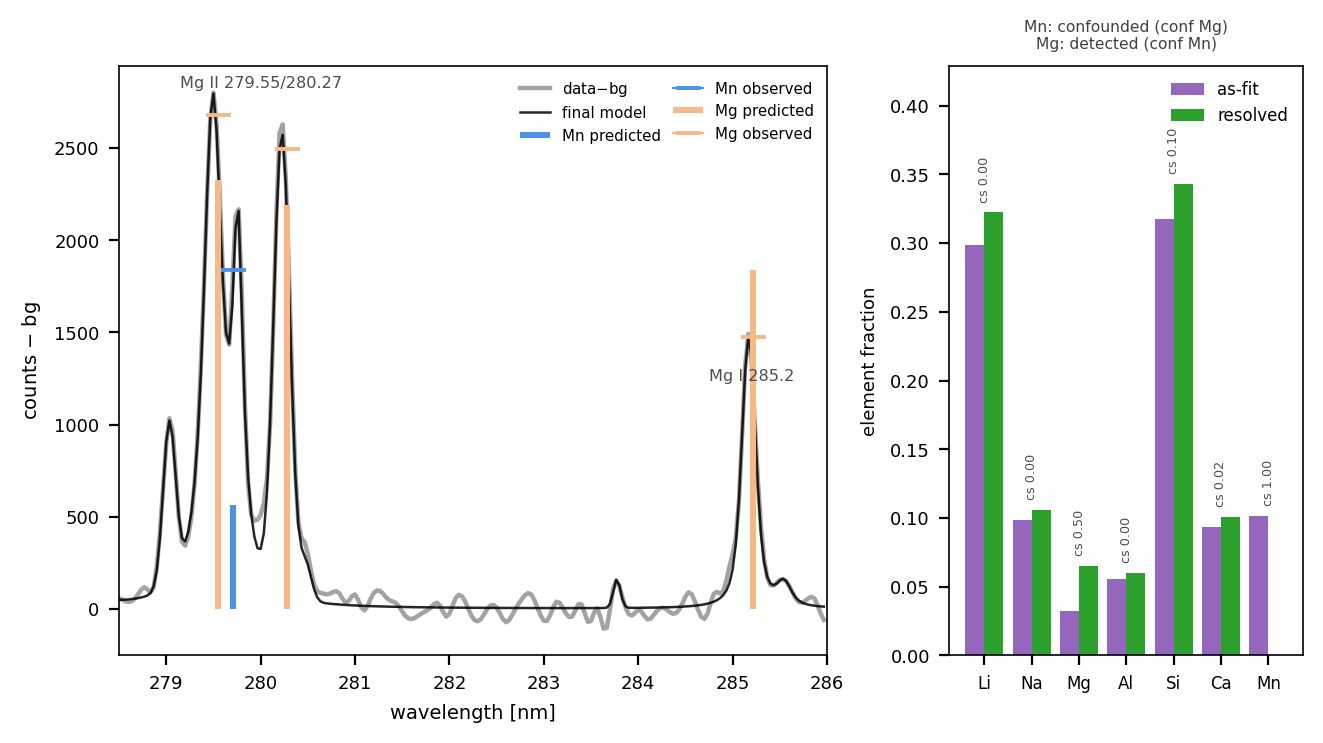
\includegraphics[width=\textwidth]{F4-confounder}
\caption{The Mn/Mg contest window (278.5--\SI{286}{\nano\metre}) of the JChristensen \texttt{MDD017-29-2c \#1} spectrum under the current adopted defaults. Left: background-subtracted data and final model; for each line that Mn or Mg claims, a stem gives that element's predicted amplitude and a bar marker the observed amplitude (areas converted to peak height). Mn's sole support line at \SI{279.76}{\nano\metre} predicts only about a third of the amplitude observed there, whereas Mg accounts for the Mg\,II 279.55/\SI{280.27}{\nano\metre} doublet and the independent Mg\,I \SI{285.2}{\nano\metre} line (which the model fits without the under-shoot seen on other spectra). Right: as-fit versus resolved fractions with the contested share (cs) above each element.
Of the 38 spectra, Mn is \texttt{confounded} on 6 and an upper limit on 10, 6 carry any \texttt{confounded} status, and the median $r^2$ is 0.78. On this spectrum ($T=\SI{9502}{\kelvin}$, $r^2=0.74$) Mn is fitted at 0.102 but its support is fully contested (cs~1.00, confounder Mg), so resolution moves Mn to 0.000 and Mg from 0.033 to 0.065. % src: manuscript/figures/cache/jc_mdd017_29_2c_1.json
\label{fig:confounder}}
\end{figure*}

\paragraph{Fit fidelity on MW2-112.}
On MW2-112 spectrum~1000, an earlier merge of asymmetric lines nearly doubled the global $\chi^2/\sigma^2$ (from 32\,821 to 51\,701) and left residuals of up to $+19\sigma$ and $40\sigma$. Replacing the merge by a nondestructive tag brought it to 28\,262, below the pre-merge value, and reduced unmodeled residuals above $3\sigma$ from 61 to 28 % src: docs/development_guide.md (Current status: ~85% complete, fit-fidelity review)
. On spectrum~0, the residual root-mean-square within merged-line windows is 2--8 times smaller for the self-absorption model than for the stored symmetric proxy for clean lines (Li~I 670.7: 227 vs 59; K~I 766.5: 101 vs 19; Fe 261.2: 141 vs 22), but is only modestly lower for a seven-component blend near \SI{383}{\nano\metre} (640 vs 549) % src: docs/fit_pipeline.md (table of merged-line residuals)
. Fit quality for blends is therefore not solved.

\paragraph{Absolute versus relative composition on MW2-112.}
In a 20-shot pilot of the closed-sum composition run, 19 nonzero spectra completed (the all-zero spectrum was correctly an error); only 3 passed quantitative physical quality control, 4 warned, and 12 failed because of low or negative $r^2$, parameters at bounds, or weak-shape and composition collapse. Doubling optimizer effort and varying the \SI{620}{\nano\metre} fallback response changed compositions substantially without stable improvement, and the 929-shot closed-sum run was rejected by the pre-registered gate % src: docs/mw2_112/analysis_plan.md (sec. 9)
. A relative-profile branch using 255 same-stage multiplets, matched-filter areas, and a requirement of at least two coherent lines per ion stage was completed for all 929 spectra. Its within-element rank correlation with the vendor summaries is 0.934 for Si, 0.883 for Ti, 0.705 for Fe, 0.657 for Li, and 0.598 for Mg, but 0.030 for Al, which is internally coherent yet externally discordant and is flagged as model limited % src: docs/mw2_112/provenance.md (Reported Spearman correlations); docs/mw2_112/analysis_plan.md (sec. 9)
. Because the vendor summaries are themselves uncalibrated, these correlations show agreement of trends, not correctness. An independent peak-window procedure supports ten elements (Al, Ba, Ca, Fe, Li, Mg, Na, Si, Sr, Ti) and rejected preliminary Ag, Cu, Ga, Ge, and V assignments as blends or single-line evidence % src: docs/mw2_112/analysis_plan.md (sec. 10)
. The output directories of these runs are not under version control.

\paragraph{A rejected physics change.}
Introducing the stimulated-emission factor into the optical depth left median $\Delta r^2$ and median change in stage disagreement at zero over 38 JChristensen spectra, yet changed alkali and Si compositions by more than 20\% in 14 of 38 samples (a control that perturbed only the optimizer trajectory did so in 3 of 38). It was refused as default because it reorients a near-degenerate alkali self-absorption and composition direction without adding information % src: docs/development_guide.md (Appendix, item 1, A/B result)
. This is an example of the acceptance logic of Section~\ref{sec:metrics}: neutral fit quality with large composition swings is instability, not accuracy.

\paragraph{Native-grid recovery.}
On the standard vendor export, which the $1/30$\,\si{\nano\metre} grid reproduces by cubic-spline resampling of the native detector pixels, the native knots were recovered to a relative residual below $10^{-6}$ in 99.1\%, 96.6\%, and 97.3\% of the NIR, VIS, and UV segments respectively across 7\,821 spectra, with a median residual of order $10^{-11}$; the \SI{0.1}{\nano\metre} export is a different product and is not covered % src: reports/2026-09-20-alibz-review.md (Moissanite archive runs table)
.

\subsection{Pure-element standards on the Z300}

Figure~\ref{fig:standard} applies the pipeline to a fresh-site iron standard on the 18-pixel-corrected native axis.

\begin{figure*}[t]
\centering
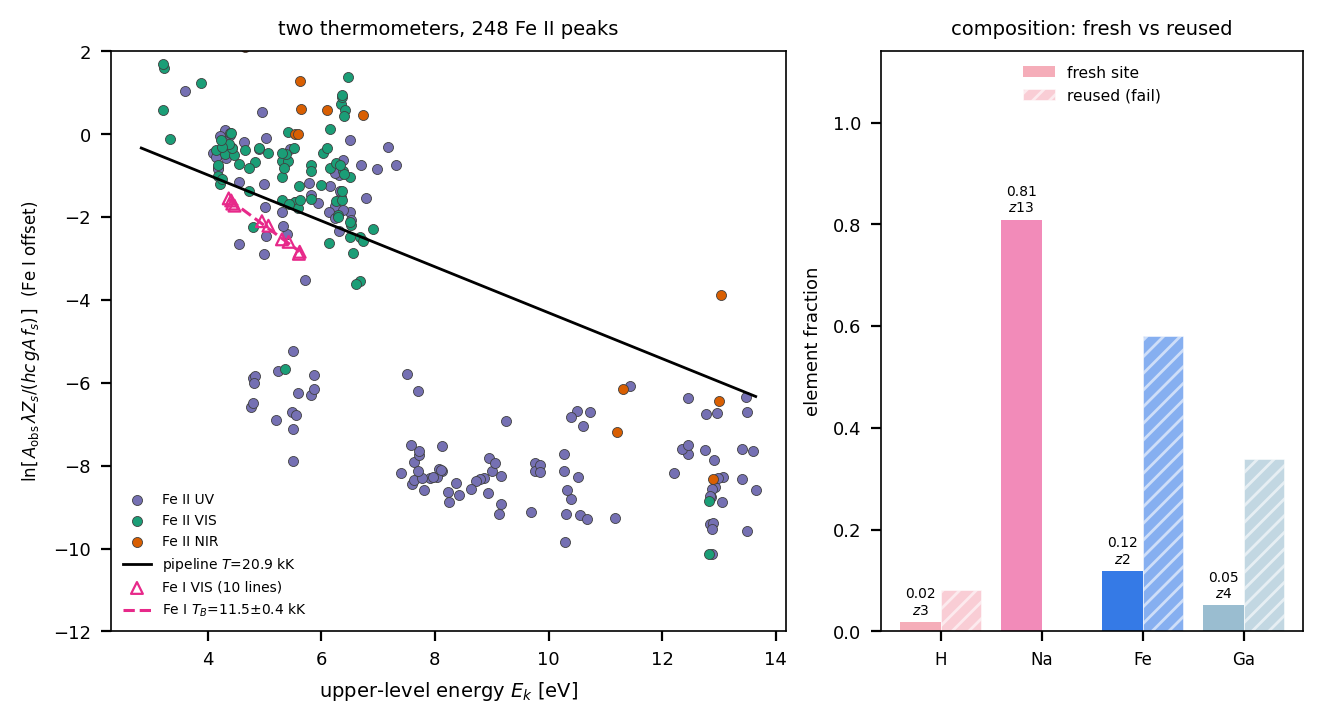
\includegraphics[width=\textwidth]{F5-standard}
\caption{Two thermometers on a pure-iron standard (\texttt{Fe\_aesar\_9998}, fresh raster site, delay 5, period 25) on the 18-pixel-corrected Z300 native axis. (a)~The whole-pattern solve's Boltzmann points, $\ln[A_{\mathrm{obs}}\,\lambda\,Z_s(T)/(hc\,gA\,f_s(T,n_e))]$ against upper-level energy $E_k$ (indexer \texttt{line\_emissivity} convention, Saha fraction $f_s$ divided out), coloured by detector segment, with the line of slope $-1/k_BT$ at the fitted $T$; the $y$-range is clipped to $[-12,2]$ (one point at $\ln\approx-20$ dropped). Overlaid are the line-selected Fe\,I visible lines (triangles, shifted vertically for display; only the slope is comparable) and their Boltzmann fit. (b)~composition, fresh (solid) versus reused spot (hatched), with detection $z$-scores.
The whole-pattern solve sits at $T=\SI{22601}{\kelvin}$ with $\log_{10}n_e=17.69$ at the upper bound of the H$\alpha$ box and assigns all 112 Fe peaks to Fe\,II (no Fe\,I), whereas the 10 isolated Fe\,I visible lines give $T_B=11.5\pm\SI{0.4}{\kilo\kelvin}$ ($r^2=0.99$, but over only a \SI{1.25}{\electronvolt} $E_k$ span, below the campaign's \SI{2.4}{\electronvolt} resolution threshold), consistent with the Fe\,I campaign median of \SI{10.8}{\kilo\kelvin}. The figure therefore documents the thermometer discrepancy on a target of known composition, not an inter-stage tie; the fresh site recovers Fe~0.93 ($z=315$, H~0.07), while the reused spot collapses to a spurious B~0.83 with Fe~0.17. % src: manuscript/figures/cache/fe_fresh_d5p25.json; manuscript/figures/cache/fe_reused_fail.json
\label{fig:standard}}
\end{figure*}

\paragraph{Axis correction.}
All Z300 native spectra were found to carry a fixed 18-pixel offset in the pixel-to-wavelength map, labeling lines about 1.6 (UV), 2.3 (VIS), and \SI{3.3}{\nano\metre} (NIR) too blue; it was identified by correlating spectra with predicted line sticks (best offsets $-18.5$, $-18.25$, and $-18.5$ pixels in the three segments) % src: reports/2026-09-23-native-axis-18px-offset.md (Finding; Evidence)
. After the correction the global shift of the Fe data is \SI{-22}{\pico\metre} (against \SI{-154}{\pico\metre} before), and a residual of about $-0.25$ pixel remains, with median manifest-recorded Ar~I offset of $-0.25$ pixel (range $-0.50$ to $+0.25$, 107 runs), varying with calibration epoch rather than constant % src: cal/reports/2026-09-24-fe-calibration-plasma-analysis.md (Wavelength shift model); reports/2026-09-24-wavelength-registration.md (Results)
. Every conclusion that depended on line identity in the earlier native analyses (registration engines, Ar anchor sets, within-segment slopes, Fe plasma temperatures, and self-absorption estimates) was repeated on the corrected axis, and only those repeated results are reported here. For example, the earlier conclusion that only three NIR Ar~I lines are argon, and the opposite-signed VIS slopes of Fe and V, were artifacts of the offset: on the corrected axis the VIS slope is about zero for both metals % src: reports/2026-09-24-wavelength-registration.md (Wavelength dependence table); docs/wavelength_registration.md (argon anchors); DECISIONS.md (2026-09-23 entries, superseded)
. Note that the 2026-09-23 entries in the decision log predate this correction.

\paragraph{Registration and drift.}
Across 107 analyzed runs (20 Fe, 87 V), element shifts are tens of picometers per segment. The best-sampled group (87 V runs over 22~h) shows a drift of about \SI{1}{\pico\metre\per\hour}, resolved statistically but physically small compared with the fixed offsets and the vendor recalibration step, so a warm-up drift hypothesis is not supported % src: reports/2026-09-24-wavelength-registration.md (Drift verdict)
. A vendor recalibration moved the Fe residual by 17--\SI{32}{\pico\metre} % src: reports/2026-09-24-wavelength-registration.md (Pre vs post the 13:39 recalibration)
.

\paragraph{Peak location.}
On 330 thin Fe lines (24 runs) in the VIS segment, the empirical point-spread-function (ePSF) estimator has a median absolute residual of \SI{5.3}{\pico\metre} against 11.2--\SI{12.3}{\pico\metre} for the vendor spline root and native parabola, with paired confidence intervals excluding zero. In the UV the spline and parabola win (4.7--\SI{4.8}{\pico\metre} against 7.6 for ePSF, on 118 thin Fe lines), and in the NIR, where there are no Fe lines, the ePSF wins on Ar~I (for 696.54~nm, 4.8 against 14--\SI{15}{\pico\metre}) but is gated to a point-Gaussian because of a sub-band seam bias % src: cal/reports/2026-09-24-empirical-lsf.md (sec. 3); alibz/data/epsf-z300-20260924.json (location blocks)
. The per-segment choice (spline in UV, ePSF in VIS, Gaussian in NIR) is therefore a measured one, and the UV and NIR entries rest on small or indirect samples.

\paragraph{Iron plasma.}
Iron-line matching on the corrected axis gives 86\% of peaks within \SI{0.15}{\nano\metre} of a database Fe line (95\% within \SI{0.40}{\nano\metre}), against 78\% and 88\% for V % src: cal/reports/2026-09-24-line-matching-sa-broadening.md (sec. 1.4)
. A Fe~I Boltzmann temperature in the visible resolves in 5 of 26 runs, giving 6873--\SI{13701}{\kelvin} (median \SI{10805}{\kelvin}) with per-run uncertainty about 15--25\%; the Fe~II UV fit resolves in none. The temperature is not detectably different across the delay/period grid (detection limit about \SI{421}{\kelvin}) and the Fe~II/Fe~I area ratio is 0.90--2.09 (median 1.49) % src: cal/reports/2026-09-24-fe-calibration-plasma-analysis.md (sec. 4 and conclusions)
. Before the axis correction the corresponding result was 8191--\SI{10451}{\kelvin} (median 9321~K) from 2 of 26 runs; the conclusion that the plasma belongs to the 8000--\SI{11000}{\kelvin} class survives, but the individual numbers do not % src: cal/reports/2026-09-24-fe-calibration-plasma-analysis.md (old versus corrected table)
. The McWhirter criterion gives only a lower bound, $\nel\ge10^{16}\,\mathrm{cm^{-3}}$ at \SI{10}{\kilo\kelvin} % src: cal/reports/2026-09-24-fe-calibration-plasma-analysis.md (4c)
, and no measured $\nel$ is reported because the cross-segment response is uncalibrated. Surface contamination (K~I) decays about 4.4-fold over the first few shots, so the first three shots on a fresh site are discarded for bulk work % src: cal/reports/2026-09-24-fe-calibration-plasma-analysis.md (discard recommendation)
.

\paragraph{Vanadium and optical depth.}
In the vanadium timing study the score falls monotonically with period at every delay (period means 1.234, 1.182, 1.119, 0.993 for periods 1, 10, 25, 50), but the V~I line signal is flat with period; the period-scaled background is a detector fixed pattern, not plasma continuum, so period acts as an exposure and the minimum period is preferred % src: cal/reports/2026-09-24-vanadium-timing-study.md (sec. 8, Q2)
. Delay is a genuine plasma lever: in an independent first run with a different site order, the V~II 311 line falls with delay at $-0.0252\pm0.0049$ per unit (5.1$\sigma$) while crater depth is not significant % src: cal/reports/2026-09-24-vanadium-timing-study.md (sec. 8, Q1)
. On the corrected axis, the temperature-independent V~I pair at 417.94/\SI{415.97}{\nano\metre} sits near its optically thin ratio (the thin value is about 2.05) and does not vary with period (its decrease with delay remains unexplained), whereas the earlier ratio of 0.75 interpreted as strong self-absorption was a misidentification caused by the offset % src: cal/reports/2026-09-24-vanadium-timing-study.md (sec. 8, Q3); reports/2026-09-23-native-axis-18px-offset.md
. This does not mean V is optically thin: the multiplet test selects seven usable V~I/II pairs, of which the strongest give optical depths of about 3.5, 1.4, and 1.4 for pairs 565.74/560.49, 653.14/645.23, and 609.02/\SI{603.97}{\nano\metre}, and 8 of 14 low-lying V~I lines lie well below the Boltzmann reference. Fe shows self-absorption on a few clean pairs (for instance 589.80/589.53 with $\tau\approx8.5$), which the earlier, misaligned analysis had found thin % src: cal/reports/2026-09-24-line-matching-sa-broadening.md (2a, 2e)
. The conclusion that pure-metal resonance lines are unsuitable as wavelength anchors, because the strongest lines are optically thick and displaced, stands from the earlier registration decision % src: DECISIONS.md (2026-09-23 independent wavelength registration)
.

\subsection{Literature-driven changes scored on a fixed panel}
\label{sec:results-ab}

Seven changes drawn from the literature of Section~\ref{sec:intro} were implemented behind
options that default off and scored, before and after, on one fixed panel: the five synthetic
suite-S scenes, the five real sample spectra, and the 26 run means of the iron standard
(Section~\ref{sec:datasets}), at the fast search settings, on one machine so that paired
comparisons are meaningful. % src: reports/2026-11-03-ab-wave1-verdicts.md; reports/fit-panel/*-moissanite.json
Table~\ref{tab:ab} gives the panel means. Huber reweighting of the concentration solve
\citep{huber1964robust} is worse on every panel. False-discovery-rate control of the element
detection score \citep{benjamini1995fdr} leaves the synthetic and real panels unchanged but
collapses the recovered iron fraction on the pure-iron standard (0.40 to 0.19) while removing the
spurious light elements, because the threshold over several hundred candidates rises above the
score of iron's own best line on runs where iron is already starved by the defect described next.
Adaptive non-negative LASSO \citep{tibshirani1996lasso,zou2005elasticnet} is neutral where it was
meant to act, since the synthetic spurious mass is already zero. The Debye correction to the
ionization energies (Section~\ref{sec:theory-saha}) is mixed. Tabulated partition functions
\citep{barklem2016partition} raise the recovered iron fraction on the standard from 0.40 to 0.56
(better on 15 of 26 runs, worse on 8) and are neutral on real spectra, but score slightly worse on
the synthetic scenes; with the Debye correction added they improve the real-spectrum $r^2$ on all
five spectra. % src: reports/2026-11-03-ab-wave1-verdicts.md

\begin{table}[t]
\centering
\footnotesize
\caption{Wave-1 panel means (fast settings; 5 synthetic, 5 real, 26 Fe-standard items; one machine).
Lower is better except $r^2$ and the Fe fraction. % src: reports/2026-11-03-ab-wave1-verdicts.md
}
\label{tab:ab}
\begin{tabular}{@{}lccccc@{}}
\toprule
Variant & Syn. median rel. err. & Syn. $|T|$ err. & Real $r^2$ & Real stage dis. & Fe fraction \\
\midrule
baseline & 0.207 & 0.082 & 0.471 & 0.515 & 0.404 \\
adaptive NN-LASSO & 0.204 & 0.081 & 0.469 & 0.467 & 0.441 \\
Huber IRLS & 0.375 & 0.197 & 0.371 & 0.496 & 0.334 \\
Debye IPD & 0.237 & 0.078 & 0.471 & 0.487 & 0.385 \\
partition tables & 0.218 & 0.085 & 0.466 & 0.491 & 0.559 \\
tables + IPD & 0.231 & 0.081 & 0.473 & 0.509 & 0.533 \\
FDR 0.05 (BH) & 0.207 & 0.082 & 0.471 & 0.515 & 0.186 \\
\bottomrule
\end{tabular}
\end{table}

The synthetic penalty of the partition tables was traced, not accepted. A scene rendered and
inverted with the same tables recovers Ca/Mg worse (median relative error 0.22) than the
line-sum pair (0.08), which a consistent forward and inverse pair should not do. The forward and
inverse models agree in emissivity space for both partition sources; the difference is in where
the plasma-state search lands. At the exact true state the inverse over-recovers Ca with either
source (0.63 line-sum, 0.71 tables, truth 0.60); the tables raise the Ca~\textsc{i} partition
function by about \SI{45}{\percent} near \SI{10}{\kilo\kelvin}, which moves the stage-consistency
minimum onto the true node where that bias is fully expressed, whereas the line-sum search lands
on a cold basin (\SI{8.9}{\kilo\kelvin}, $\log_{10}\nel=16.5$) where the bias is accidentally
compensated. % src: reports/2026-11-03-debug-partition-roundtrip.md
The bias itself was then isolated to the design matrix. Each database line's predicted emission
is spread over every fitted peak within the \SI{0.1}{\nano\meter} shift tolerance by a Voigt
height ratio, so one line can be counted against several peaks and a dense-forest element is
over-predicted per unit concentration in proportion to how often its lines fall near two fitted
components. With a fitter-realistic oracle (the forward model's own line areas, lines closer than a
quarter of the instrumental width merged into one peak as a fitter would merge them) solved at the
exact true state, the legacy map returns Si 0.31 and Ca 0.37 on the silicate scene (truth 0.40 and
0.30), whereas assigning each line to the single fitted component under it, so that a component is
the sum of the database lines it covers, returns 0.36 and 0.27; on the binary scene the two maps
give Ca 0.61 and 0.60. A clean control $\mathbf{y}=\mathbf{A}\mathbf{c}_\mathrm{true}$ is exact
under the hard assignment but not under the legacy map, which is therefore inconsistent even on
its own data. % src: reports/2026-11-04-candidate-coverage.md (merged oracle tables); reports/2026-11-03-wave2-conserving-design.md
The same oracle exposed a second, independent gap: iron is recovered at 0.27 (truth 0.20) under
either map because the design matrix under-predicts the generator's iron areas by about a factor
1.23 relative to the other elements at the same plasma state, so the solve inflates iron to
compensate; the per-element aggregation itself is exact on a clean control. The source of that
iron-specific forward-versus-inverse disagreement is being isolated. % src: reports/2026-11-04-aggregation-floor.md
Both the conserving and the hard-assignment maps were implemented as options and scored in a
second round together with the partition tables and the Debye correction, against a baseline built
from the same code (the panel is deterministic: identical code reproduces every metric). The
hard assignment is exact at the true state and clean of spurious species, but end to end, at the
fast search settings, it scores worse than the baseline on the synthetic median error (0.208 against
0.156) because the unweighted solve absorbs iron's line-shape misfit; the conserving map combined
with the tables and the Debye correction is the only variant that improves the mean of every
headline on all three panels. % src: reports/2026-11-04-ab-wave2-verdicts.md
Against the true baseline (a bisection found and gated two changes that had altered the default
path unflagged during the round, so every earlier comparison was re-run) the combination improves
every headline mean: synthetic median relative error 0.207 to 0.156 (better on three of five
scenes), temperature error 0.082 to 0.069, real-spectrum $r^2$ 0.471 to 0.478 and stage
disagreement 0.515 to 0.500 (each better on four of five spectra), and the iron fraction on the
pure-iron standard 0.40 to 0.55 (better on 13 of 26 runs). At the production search settings
the gains persist (synthetic median relative error 0.213 to 0.170, real $r^2$ 0.472 to 0.488,
iron fraction 0.43 to 0.56) with two costs we record: one synthetic scene's dominant element is
no longer identified correctly, and the spurious-element count on the iron standard rises
slightly (0.96 to 1.08), both within the paired noise of five- and 26-item panels. % src: reports/2026-11-04-ab-wave2-verdicts.md (series 3 + prod2); reports/fit-panel/{head,cpi}-prod2.json; DECISIONS.md 2026-11-04 addendum
These three options are now the pipeline defaults; the weighted solve with hard assignment, which
recovers every major of the silicate scene within 0.01 at the true state, remains an option
because its search misbehaves away from the true state.
A third round scored three further model changes behind flags, each against a baseline re-run on
the same tree. The overlap kernel was given each peak's own fitted width and each database line
its own Stark width at the trial electron density; at the fast search settings this variant lifted
the primary headline of every panel, but at the production settings it is mixed (real-spectrum
$r^2$ 0.489 to 0.509, better on four of five spectra, and the mis-identified dominant element of
the binary scene repaired, against synthetic median relative error 0.170 to 0.174 and iron fraction
0.563 to 0.545, worse on 14 of 26 runs), so it remains an option. The same round showed that the
merged oracle cannot arbitrate a width kernel at all, because its peaks sit on their own line
centres where every width gives unit overlap; only the end-to-end panel can. A bounded local polish
of the plasma state after the Bayesian search was rejected: a Powell polish within the budget is a
near no-op, and a Nelder--Mead polish lowers the outer objective by 10 to 60\% on the synthetic
scenes yet moves the temperature away from the truth, which says that the objective's minimum is
not at the true state and that a better search would not help until the model is. A two-temperature
stage thermometer (ion stages at $T+\delta$, $0 \le \delta \le 2000$~K) was rejected because
$\delta$ pins to its bound on three of five single-temperature synthetic scenes and doubles the
synthetic temperature error, and a per-species McWhirter gap flag changed no item on the panel
because the species it flags carry no multi-stage support. % src: reports/2026-11-04-w3-width-kernel.md; reports/2026-11-04-w3-outer-polish.md; reports/2026-11-04-w3-thermometer.md; reports/fit-panel/w3k-peakstark-conserve-prod.md

\subsection{Known failure modes}

The following failure modes were observed and are either guarded or flagged. None is claimed to be eliminated.

\begin{description}
\item[Basin collapse.] A re-index seeded with many weak low-excitation lines drifted into a low-temperature basin (about \SI{5200}{\kelvin}) where one element's small Saha--Boltzmann response explained everything, giving Hg~1.000 from a single \SI{194}{\nano\metre} line, Fe~0.991, and Ca~0.990 on JChristensen spectra, while $r^2$ rose to 0.87. A guard rejects a re-solve whose top fraction newly reaches 0.9 % src: docs/development_guide.md (honest measured caveat); alibz/pipeline.py (COLLAPSE_TOP_FRACTION comment)
.
\item[Phantom single-line elements.] Bi was reported at 0.94 when its strongest predicted line was 4 counts % src: docs/development_guide.md (A zero-emission species dominated the composition)
; in MW2-112, preliminary Ag, Cu, Ga, Ge, and V assignments were rejected as blends or single-line evidence % src: docs/mw2_112/analysis_plan.md (sec. 10)
. In a 99.98\% Fe target, almost every trace line lies near an Fe line, and several candidate trace detections (Ca~II, Ca~I) were downgraded to Fe-blends % src: cal/reports/2026-09-24-fe-calibration-plasma-analysis.md (sec. 1 table, limits)
.
\item[Confounders.] Mn$\leftrightarrow$Mg as above; a corpus-level catalog aggregates recurring pairs. An element whose all support is contested is an attribution choice, not a measurement.
\item[$\nel$ at bound.] The data lean cold along the Saha ridge, so the search sits at the low edge of whatever $\nel$ box it is given; for the reported vendor export the search ended at the H$\alpha$ edge and the exported flag \texttt{electron-density-at-bound} was set, together with \texttt{dominant-weak-shape} and \texttt{detector-response-fallback} % src: reports/2026-09-21-stage-consistency-thermometer.md (sec. 3 and sec. 4)
.
\item[Alkali resonance lines.] Rigid doublet-ratio vetoes are unsafe: 926 of 928 measured K pairs fall outside $\pm20\%$ of the thin ratio on the examined data, and K and Na compositions move by 30--60\% on real spectra with the self-absorption degeneracy % src: DECISIONS.md (2026-09-22 Early Ar/O diagnostics); docs/development_guide.md (Appendix item 1)
.
\item[Axis offset.] A fixed 18-pixel offset silently mis-assigned elements in all native Z300 data until 2026-09-24; an Ar~I cross-correlation check now records an axis warning in the acquisition record when the offset exceeds two pixels or the lock is ambiguous (it does not reject the data) % src: reports/2026-09-24-pixel-offset-fix.md (acquire.py axis check)
. Results from before the correction are superseded.
\end{description}

\subsection{Summary of evidence and gaps}

The evidence to date supports three statements. The inverse model, with the stage-consistency thermometer and an $\nel$ box, recovers the temperature and dominant composition of Saha-consistent synthetic scenes at the level of the pinned tolerances and moves real spectra to physically more plausible states. Confounded and collapsed solutions are detected and flagged, and some are resolved. And on pure-element standards the corrected axis, the line identifications, and a visible-range Boltzmann temperature are consistent with a plasma of roughly 7--\SI{14}{\kilo\kelvin}. The evidence does not yet support any statement about composition accuracy on real samples, the relative merit of the two inverse engines, or invariance to argon versus air. Those require certified reference materials, a re-run of the benchmark, and a dedicated paired acquisition, respectively (Section~\ref{sec:datasets}).

\section{Discussion}
\label{sec:discussion}

\subsection{What a physics-first inverse model buys}

The central argument of this paper is not that \alibz{} is more accurate than
calibrated or learned methods; Section~\ref{sec:results} shows that the absolute,
closed-sum quantification of heterogeneous single shots is not yet reached. The
argument is that an inverse model built from Equations~\eqref{eq:emissivity},
\eqref{eq:saha} and \eqref{eq:wnnls} fails in ways that can be seen. Every failure
mode documented in Section~\ref{sec:results} was caught by a diagnostic that the
model itself produces: a basin collapse appears as a top fraction that jumps to one
while $r^2$ \emph{improves}; a confounded attribution appears as a supporting peak set
that a rival could cover at its own true-negative cap (Equation~\eqref{eq:contest});
a phantom trace element appears as a detection score $z<3$ on its strongest predicted
line (Equation~\eqref{eq:detect}); a wrong plasma state appears as a stage
disagreement $D_\mathrm{el}$ (Equation~\eqref{eq:stage-disagreement}) or an electron
density pinned to the edge of its prior box. A purely empirical regressor
\citep{clegg2009pls,li2020cnn} returns a composition in each of these cases with no
residual structure to flag it, because nothing in the model is obliged to be
consistent with Saha--Boltzmann physics. That is the sense in which the assumptions of
Section~\ref{sec:assumptions} are an asset rather than a liability: the ones that
matter are tested at run time, and the ones that are not yet tested are named.

\subsection{Where the model is limited by physics, and where by the instrument}

Two limitations are intrinsic to the measurement and no amount of software removes
them. The first is the weak information that line amplitudes carry about the plasma
state. The amplitude objective is flat in $\nel$ at fixed $T$ and nearly flat in $T$
over several thousand kelvin (Section~\ref{sec:theory-thermometer}), so the
composition of a feldspar-like spectrum, whose Si/K emissivity ratio changes by a
factor of $\sim$2.5 per \SI{1000}{\kelvin}, is only as good as the thermometer and
the density anchor. The stage-consistency cost fixes $T$ where two stages of one
element are observed, and H$\alpha$ fixes $\nel$ where hydrogen is present
\citep{gigosos2003halpha}; otherwise \alibz{} falls back to a prior and says so. This
is the same identifiability problem that limits classical CF-LIBS Boltzmann and
Saha--Boltzmann plots \citep{tognoni2010cflibs,aguilera2007multielement}, made
explicit by treating the stages as independent unknowns rather than hidden by tying
them. The second intrinsic limitation is spatial and temporal inhomogeneity
\citep{aragon2008review,cristoforetti2013columnar}: a single $(T,\nel)$ is an
effective average over a gated, expanding plasma, and on a multi-phase mineral the
same element is excited in different host phases. The stage disagreement is the
diagnostic for both, and it cannot separate them; correlative characterization of the
ablated phases is the only route to doing so.

Three further limitations belong to the instrument and are therefore removable. The
relative spectral response within and between the ultraviolet and visible segments is
uncalibrated (Assumption~A6), and the \SI{620}{\nano\meter} gain step is measured
from the continuum with a corpus fallback; on feldspar-like spectra the K/Si split is
limited by that fallback, not by the thermometer. A lamp calibration and a
branching-ratio method \citep{li2014spectralresponse,urbinamedina2021branching} are
the planned fixes. The line-spread function is not a Voigt, the vendor export grid is
a spline resample of coarser native pixels, and the pipeline now fits on the native
grid with per-segment location estimators (Section~\ref{sec:wf-fit}); a
forward-convolved, pixel-integrated line-spread function remains to be built, and
until it is, the self-absorption parameters of Equation~\eqref{eq:sa-voigt} partly
absorb instrument shape (Assumption~A9). Finally, the wavelength axis carried an
18-pixel offset that invalidated every line identification made before it was found
(Section~\ref{sec:results}); the per-spectrum registration against ambient argon
lines now bounds the residual to a fraction of a pixel, but it is a reminder that an
instrument-level error can masquerade as physics.

Atomic data are a limitation of a third kind. Transition probabilities enter
Equation~\eqref{eq:emissivity} linearly and carry accuracy classes from a few percent
to \SI{50}{\percent} \citep{kramida2023asd,fuhr2006fe}; partition functions are
summed from the line-derived level set rather than taken from critically evaluated
tables \citep{barklem2016partition}; ionization-potential depression and the
McWhirter criterion are not evaluated (Section~\ref{sec:theory-saha}). None of these
is tested at run time. They set a floor on the accuracy that any calibration-free
method can reach, and the synthetic generator samples them as source-aware
uncertainty precisely so that a trained model does not learn to trust them.

\subsection{The MW2-112 production gate}

The clearest statement of where the method stands is the pre-registered production
gate of the MW2-112 stratigraphic profile (Section~\ref{sec:datasets}). The
closed-sum CF-LIBS branch was rejected: in the 20-shot quantitative pilot only 3
positions passed the physical quality control, 4 warned and 12 failed on low or
negative pattern $r^2$, plasma parameters at bounds, or weak-shape and composition
collapse, and doubling the optimizer effort or varying the \SI{620}{\nano\meter}
fallback response changed the compositions without stable improvement.
% src: docs/mw2_112/analysis_plan.md §9 (execution record 2026-07-15)
A relative-profile branch, which asks only for within-element spatial ranks from
same-stage multiplets, was completed for all 929 spectra and validates against the
vendor's independent summaries (Spearman $\rho$ of 0.93 for Si, 0.88 for Ti, 0.71 for
Fe, 0.66 for Li and 0.60 for Mg).
% src: docs/mw2_112/analysis_plan.md §9
The contrast is instructive: the forward model and the peak-extraction chain are
good enough to rank, and the identification and plasma-state inference are the
weak links for absolute quantification on single shots of a heterogeneous,
finely stratified mudrock. The calibration campaign on pure-element standards
(Section~\ref{sec:datasets}) was begun for exactly this reason: on a target whose
composition is known, every residual is attributable to the instrument or the
physics rather than to the sample.

\subsection{What the panel taught: basins compensate, matrices must conserve}

Two lessons from Section~\ref{sec:results-ab} generalise beyond the specific changes. First, a
physically more correct ingredient can score worse on a round trip when the baseline's error is
being cancelled by a second error: the line-sum partition function landed the search on a cold
basin that compensated a composition bias, and the tabulated functions were penalised for
removing the compensation. A fixed panel with a solve at the known true state is what exposed
this; a benchmark that only reports end-to-end accuracy would have rejected the correct physics.
Second, the whole-pattern design matrix must conserve emission. Spreading one database line over
several nearby peaks is a natural way to tolerate wavelength error, but it lets one line be
counted against two fitted components, which over-predicts the elements whose lines most often
have a second component within the tolerance, and the non-negative solve then under-recovers
them; on the silicate scene that is silicon, and on real spectra it is likely to be iron, whose
forest is the densest. The principled alternative is to let each fitted component be the sum of
the database lines under it. This is a property of the inverse model, not of the plasma, and
it is invisible to goodness of fit. We expect it to account for part of the single-element
dominance failures of Section~\ref{sec:results} and for the pure-iron standard's low iron
fraction; the conserving matrix is therefore the first change of the next round, and the
candidates already scored are re-evaluated on top of it rather than on the biased solver.

\subsection{Relation to learned models}

We regard the physics-first inverse model and the learned models of
Section~\ref{sec:intro} as complementary rather than competing, in two concrete
ways. First, the forward model is the source of labelled training data. The
explicit-stage synthetic generator (Section~\ref{sec:datasets}) renders spectra with
independent stage abundances, per-stage temperatures and source-aware atomic
uncertainty onto arbitrary pixel grids, and the planned coordinate-aware transformer
is specified to be trained on it, with acceptance gates on conditional peak-profile
and export-kernel realism before training begins. Randomizing the simulator in this
way is the established route to transfer from synthetic to real data
\citep{tobin2017domainrand}, and set- and point-based attention
\citep{lee2019settransformer,zaheer2017deepsets} is the natural architecture for
irregularly sampled, multi-segment spectra. Second, the inverse model supplies the
consistency checks that a learned model lacks: a network's composition can be
forward-modelled at its implied plasma state and scored by the same residual, stage
disagreement and detectability diagnostics as a solver's. Physics-informed training
\citep{raissi2019pinn} embeds the same equations as penalties; the difference is
whether the physics is a constraint on the answer or a diagnostic of it, and we
argue for keeping both.

A more immediate statistical improvement is already identified. Comparing basins by
$r^2$ fails because a degenerate single-element basin can fit a noisy spectrum
better than the truth (Section~\ref{sec:results}); whitening the objective by a
per-peak noise model (Equation~\eqref{eq:sigma-eff}) repairs the comparison on
synthetic scenes but remains opt-in because its $\chi^2$ still misranks
temperature. A pixel-level likelihood with a parametric, positive-definite noise
covariance, replacing the peak table as the solver's input, is the fundamental fix;
its prototype showed that correlated-noise whitening on the resampled export grid
rewards sharp features and must be paired with the native grid and a noise nugget.

\subsection{Open validation gates}

Three gates remain open, in order of what they would establish. (i)
\emph{Composition invariance}: the same rock measured under argon and in air must
return the same composition while $T$ and $\nel$ differ \citep{palasti2022argon};
the metric is defined (Section~\ref{sec:metrics}) but no measured pair has yet been
staged into the repository, so it has been exercised only on a synthetic argon-ambient
scene. (ii) \emph{Pure-element standards}: the Z300 iron and vanadium studies
constrain the plasma temperature, the doublet optical depths and the wavelength
registration, but a pure metal cannot test the composition solve. (iii)
\emph{Certified reference materials}: no certified geological or glass standard
\citep{jochum2005georem,jochum2011nist} has yet been measured; the benchmark
scaffolding carries placeholders for them, and the working accuracy target is a
relative error on major elements of about \SI{20}{\percent}.
% src: DECISIONS.md 2026-11-03 entry recording the 2026-07-01 target
Until (iii) is passed, every accuracy statement about \alibz{} rests on synthetic
round trips, whose noise and atomic data are, by construction, those of the model.

\section{Conclusions}
\label{sec:conclusions}

We have set out the theoretical basis, the assumptions, the processing workflow,
the datasets and the fit metrics behind \alibz, an open-source toolkit for
calibration-free quantification of laser-induced breakdown spectra by
whole-pattern forward modelling. The model is a non-negative linear combination
of Saha--Boltzmann element--ion templates evaluated at a shared plasma state, with
a single line-intensity convention shared by the forward and inverse directions,
independent ion stages whose disagreement is reported rather than suppressed, a
stage-consistency thermometer that fixes the temperature where amplitudes cannot,
Balmer-line Stark widths or an explicit prior for the electron density, and
self-absorption handled by resolved-profile fits and doublet-ratio inversion. The
inverse solve is guarded by a noise-relative detectability gate, a basin-collapse
guard and a true-negative contest that resolves spectral confounders.

Eleven assumptions are stated with their status. Those that most often fail
silently in calibration-free LIBS, namely optical thinness, single-plasma stage
consistency, confounded attribution and wavelength registration, are tested at
run time; the local-thermodynamic-equilibrium criterion, the absolute spectral
response, the atomic-data accuracy and the line-spread shape are not yet tested
and are named as such. On synthetic spectra the method recovers temperature,
composition and, when anchored, electron density; on real single shots of a
heterogeneous lithium mudrock the closed-sum quantification was rejected by its
own pre-registered gate while the relative element profiles validated against
independent measurements; and on pure-element standards measured with a handheld
analyser the plasma temperature, the resonance-doublet optical depths and the
wavelength registration are now characterised on a corrected axis.

A first literature-driven round, scored on a fixed panel with a solve at the known true state as
well as end to end, exposed and corrected a replication defect in the whole-pattern design matrix
and adopted tabulated partition functions and the Debye ionization-potential correction as
defaults; it also showed that a physically correct ingredient can be penalised by a round trip when
a compensating error is removed, which is why the panel keeps a solve at the known state.
The open gates are explicit: composition invariance between argon and air,
pure-element standards for the plasma physics, and certified reference materials
for the composition solve. The same forward model that underlies the solver is the
training-data source for a planned synthetic-trained transformer, and the
diagnostics defined here are intended to score that model on the same footing.
Every number in this paper carries, in the source of the manuscript, the path of
the report, test or notebook that produced it, and the repository that produced
them is public.


\section*{Acknowledgements}
\todo{funding, instrument access (SciAps Z300), compute (moissanite, beryl), collaborators.}

\section*{Data and code availability}
\alibz{} is open source at \url{https://github.com/MWhitta/alibz}. \todo{DOI for the
tagged release; dataset deposition for the spectra used here.}

\bibliographystyle{unsrtnat}
\bibliography{bib/theory,bib/cflibs,bib/ml,bib/local}

\appendix
\section{Notation}
\label{app:notation}

\begin{table}[h]
\centering
\small
\begin{tabular}{@{}llp{0.58\linewidth}@{}}
\toprule
Symbol & Units & Meaning \\
\midrule
$T$ & K & excitation (and, under A1, ionization) temperature of the plasma \\
$\nel$ & cm$^{-3}$ & electron density; carried internally as $\log_{10}\nel$ \\
$z$ & -- & ionization stage ($z=1$ neutral) \\
$N_z$, $f_z$ & cm$^{-3}$, -- & number density of an element in stage $z$ and its fraction, Eq.~\eqref{eq:stage-fraction} \\
$U_z(T)$ & -- & partition function of stage $z$, Eq.~\eqref{eq:partition} \\
$g_k$, $E_k$ & --, eV & statistical weight and energy of level $k$; $E_i$ the lower level of a line \\
$gA_j$ & s$^{-1}$ & $g_kA_{ki}$ of line $j$ (database transition strength) \\
$\chi_z$ & eV & ionization energy from stage $z$ to $z+1$ \\
$\lambda_j$ & nm & air wavelength of line $j$ (vacuum below \SI{200}{\nano\meter}) \\
$\varepsilon_j(T,\nel)$ & eV\,sr$^{-1}$ & line emissivity per emitter, Eq.~\eqref{eq:emissivity} \\
$R(\lambda)$ & -- & instrument spectral response, Eq.~\eqref{eq:forward-line} \\
$\sigma$, $\gamma$ & nm & Gaussian standard deviation and Lorentzian half-width of a Voigt profile \\
$\tau$, $\tau_a$, $\delta$ & --, --, nm & optical depth; cold-absorber depth and shift in Eq.~\eqref{eq:sa-voigt} \\
$\kappa_j$, $s_\tau$ & -- & per-line absorption factor and global optical-depth scale, Eq.~\eqref{eq:kappa} \\
$f_\mathrm{SA}(\tau)$ & -- & escape factor $(1-e^{-\tau})/\tau$, Eq.~\eqref{eq:escape} \\
$R_0$, $s_r$ & -- & optically thin doublet ratio and absorption-strength ratio, Eq.~\eqref{eq:doublet} \\
$\mathbf{A}(T,\nel)$ & counts & design matrix, one column per (element, stage) template \\
$\mathbf{y}$, $\mathbf{c}$ & counts, -- & observed peak areas and non-negative concentrations, Eq.~\eqref{eq:wnnls} \\
$\sigma_{\mathrm{eff},j}$ & counts & effective per-peak area uncertainty, Eq.~\eqref{eq:sigma-eff} \\
$z_\mathrm{det}$ & -- & detection score of an element's strongest predicted line, Eq.~\eqref{eq:detect} \\
$D_\mathrm{el}$ & -- & stage disagreement, Eq.~\eqref{eq:stage-disagreement} \\
$C_\mathrm{tie}$ & counts$^2$ & stage-consistency (thermometer) cost, Eq.~\eqref{eq:tie-cost} \\
$c_\mathrm{max}(E')$ & -- & true-negative cap on a rival element in the confounder contest, Eq.~\eqref{eq:contest} \\
\bottomrule
\end{tabular}
\end{table}

\section{Pipeline parameters and defaults}
\label{app:params}

Tables~\ref{tab:params-fit}--\ref{tab:params-solve} list the defaults of the \alibz\ pipeline as they stand in the code at the time of writing. Each parameter is named as it appears in the module given in the second column; entries marked ``literal'' are numerical constants inside a function body and not named constants. Quantities written with an exponent or a subscript are given in plain text for compatibility with the code. Parameters in Section~\ref{sec:workflow} that are not listed here (for example the stage tolerances of the golden-line selector) are internal and are not intended to be tuned.

\begin{table*}[!htbp]
\centering
\caption{Background, detection and profile fitting.}
\label{tab:params-fit}
\scriptsize
\setlength{\tabcolsep}{4pt}
\begin{tabular}{@{}p{0.09\textwidth}p{0.17\textwidth}p{0.24\textwidth}p{0.13\textwidth}p{0.28\textwidth}@{}}
\toprule
Stage & Module & Parameter & Default & Meaning \\
\midrule
Background & \texttt{peaky\_\allowbreak{}finder} & \texttt{DEFAULT\_\allowbreak{}SEGMENT\_\allowbreak{}EDGES} & (365.0, 620.0) nm & Detector junctions at which the spectrum is split for background, noise and fits \\
Background & \texttt{peaky\_\allowbreak{}finder} & \texttt{smooth\_\allowbreak{}nm} & 1.9 nm & Physical arPLS smoothing length; the penalty weight is $(\ell/\Delta\lambda)^4$ \\
Background & \texttt{peaky\_\allowbreak{}finder} & \texttt{max\_\allowbreak{}iter} & 20 & arPLS reweighting iterations \\
Detection & \texttt{peaky\_\allowbreak{}finder} & \texttt{n\_\allowbreak{}sigma} & 0 & Added to the 3.0 $\sigma$ floor of the local noise; cannot loosen it \\
Detection & \texttt{peaky\_\allowbreak{}finder} & \texttt{\_\allowbreak{}noise\_\allowbreak{}scale\_\allowbreak{}local block} & 2048 samples & Block length of the robust noise estimate; blocks restart at junctions \\
Fitting & \texttt{peaky\_\allowbreak{}finder} & \texttt{MIN\_\allowbreak{}HEIGHT\_\allowbreak{}SIGMA} & 2.0 & Final gate: implied height must exceed this multiple of local noise \\
Fitting & \texttt{peaky\_\allowbreak{}finder} & \texttt{fit\_\allowbreak{}all window} & 50 samples & Half-width of the joint block refit (literal in code) \\
Fitting & \texttt{peaky\_\allowbreak{}finder} & \texttt{width filter} & 100 $\times$ median FWHM & Components wider than this are discarded as baseline remnants (literal in code) \\
\bottomrule
\end{tabular}
\end{table*}

\begin{table*}[!htbp]
\centering
\caption{Refinement, deblending and self-absorption.}
\label{tab:params-refine}
\scriptsize
\setlength{\tabcolsep}{4pt}
\begin{tabular}{@{}p{0.09\textwidth}p{0.17\textwidth}p{0.24\textwidth}p{0.13\textwidth}p{0.28\textwidth}@{}}
\toprule
Stage & Module & Parameter & Default & Meaning \\
\midrule
Refinement & \texttt{refinement} & \texttt{BIC\_\allowbreak{}MARGIN} & 10.0 & BIC margin for a database-supported blend verdict \\
Refinement & \texttt{refinement} & \texttt{BIC\_\allowbreak{}MARGIN\_\allowbreak{}UNSUPPORTED} & 30.0 & BIC margin for a blend without database support \\
Refinement & \texttt{refinement} & \texttt{TAU\_\allowbreak{}MAX} & 8.0 & Absorber optical-depth ceiling; a fit at the ceiling is never acted on \\
Refinement & \texttt{refinement} & \texttt{SA\_\allowbreak{}ROBUST\_\allowbreak{}F\_\allowbreak{}SCALE} & 8.0 & Scale of the soft-L1 robust loss \\
Refinement & \texttt{refinement} & \texttt{s2\_\allowbreak{}action\_\allowbreak{}max} & 50.0 & Decisions whose noise rescale exceeds this are recorded, not applied \\
Refinement & \texttt{refinement} & \texttt{resonance gate} & E\_i $\le$ 0.2 eV & Lower-level energy for a resonance-capable (self-absorbing) primary line (literal in code) \\
Deblending & \texttt{profiles} & \texttt{DEBLEND\_\allowbreak{}ACCEPT\_\allowbreak{}SNR} & 4.0 & Matched-filter signal-to-noise ratio to accept a shoulder deblend \\
Deblending & \texttt{profiles} & \texttt{DEBLEND\_\allowbreak{}BIC\_\allowbreak{}MARGIN} & 6.0 & Window BIC margin for a deblend \\
Deblending & \texttt{profiles} & \texttt{DEBLEND\_\allowbreak{}MAX} & 12 & Maximum new components per spectrum \\
SA recovery & \texttt{profiles} & \texttt{SA\_\allowbreak{}BIC\_\allowbreak{}MARGIN} & 10.0 & BIC win required over the symmetric control \\
SA recovery & \texttt{profiles} & \texttt{SA\_\allowbreak{}AMPLIFICATION\_\allowbreak{}CAP} & 5.0 & Maximum emission-to-observed area ratio accepted \\
\bottomrule
\end{tabular}
\end{table*}

\begin{table*}[!htbp]
\centering
\caption{Registration, seeding and deepening.}
\label{tab:params-seed}
\scriptsize
\setlength{\tabcolsep}{4pt}
\begin{tabular}{@{}p{0.09\textwidth}p{0.17\textwidth}p{0.24\textwidth}p{0.13\textwidth}p{0.28\textwidth}@{}}
\toprule
Stage & Module & Parameter & Default & Meaning \\
\midrule
Registration & \texttt{pipeline} & \texttt{wavelength\_\allowbreak{}registration} & ambient & Mode: off, report, ambient or apply\_element \\
Registration & \texttt{pipeline} & \texttt{subpixel} & gaussian & Sub-pixel center method: gaussian or parabolic \\
Registration & \texttt{pipeline} & \texttt{gas\_\allowbreak{}wavelength\_\allowbreak{}calibration} & apply & Independent Ar I / O I engine: off, report or apply \\
Registration & \texttt{wavelength\_\allowbreak{}registration} & \texttt{SEGMENT\_\allowbreak{}EDGES} & (365.0, 620.0) nm & Segment junctions for registration \\
Registration & \texttt{wavelength\_\allowbreak{}registration} & \texttt{golden-line minimum} & 3 lines & Fewer golden lines leave a segment unregistered (documented in code) \\
Registration & \texttt{wavelength\_\allowbreak{}registration} & \texttt{isolation\_\allowbreak{}window\_\allowbreak{}nm} & 0.30 nm & Search window for isolation of element anchors \\
Registration & \texttt{wavelength\_\allowbreak{}registration} & \texttt{kT\_\allowbreak{}eV} & 0.78 eV (9000 K) & Boltzmann temperature that ranks golden-line strength \\
Segment shift & \texttt{utils.wavelength} & \texttt{MIN\_\allowbreak{}SHIFT\_\allowbreak{}MATCHES} & 5 & Minimum unambiguous matches for a segment's own median \\
Segment shift & \texttt{utils.wavelength} & \texttt{significance gate} & 2 $\times$ SE & A segment median is adopted only beyond this multiple of its standard error (literal in code) \\
Seeding & \texttt{minor\_\allowbreak{}lines} & \texttt{DEFAULT\_\allowbreak{}KT\_\allowbreak{}EV} & 0.76 eV & Single reference temperature for Boltzmann ratios \\
Seeding & \texttt{minor\_\allowbreak{}lines} & \texttt{tol\_\allowbreak{}nm} & 0.06 nm & Match tolerance between database and fitted peak \\
Seeding & \texttt{minor\_\allowbreak{}lines} & \texttt{min\_\allowbreak{}ref\_\allowbreak{}lines} & 3 & Consistent references needed for a stage to predict \\
Seeding & \texttt{minor\_\allowbreak{}lines} & \texttt{max\_\allowbreak{}scale\_\allowbreak{}spread} & 0.6 & Maximum relative spread of the stage scale \\
Seeding & \texttt{minor\_\allowbreak{}lines} & \texttt{min\_\allowbreak{}ref\_\allowbreak{}snr} & 10.0 & Minimum signal-to-noise ratio of a reference line \\
Seeding & \texttt{minor\_\allowbreak{}lines} & \texttt{consistency\_\allowbreak{}factor} & 5.0 & Agreement with the Boltzmann prediction required to add a line \\
Seeding & \texttt{minor\_\allowbreak{}lines} & \texttt{bic\_\allowbreak{}margin} & 2.0 & BIC improvement required for an added line \\
Recovery & \texttt{minor\_\allowbreak{}lines} & \texttt{snr\_\allowbreak{}min} & 4.0 & Local-noise bar for element-agnostic residual recovery \\
Recovery & \texttt{minor\_\allowbreak{}lines} & \texttt{bic\_\allowbreak{}margin (recovery)} & 6.0 & BIC margin for a recovered line \\
Recovery & \texttt{minor\_\allowbreak{}lines} & \texttt{max\_\allowbreak{}new} & 40 & Maximum recovered lines per call \\
Deepening & \texttt{pipeline} & \texttt{CONFIDENT\_\allowbreak{}MIN\_\allowbreak{}REFS} & 4 & Clean reference lines for an ion to be confident \\
Deepening & \texttt{pipeline} & \texttt{DEEPEN\_\allowbreak{}BARS} & (3.0, 2.0) $\sigma$ & Successive local-noise bars for the deepening rounds \\
Deepening & \texttt{pipeline} & \texttt{SUPPORT\_\allowbreak{}GA\_\allowbreak{}FLOOR} & 1e6 & gA floor for a database line that marks coverage \\
Deepening & \texttt{pipeline} & \texttt{SUPPORT\_\allowbreak{}TOL\_\allowbreak{}NM} & 0.06 nm & Position tolerance for that coverage \\
Deepening & \texttt{pipeline} & \texttt{ESTABLISHED\_\allowbreak{}MIN\_\allowbreak{}FRACTION} & 0.002 & Pass-1 fraction above which an element seeds minor lines \\
\bottomrule
\end{tabular}
\end{table*}

\begin{table*}[!htbp]
\centering
\caption{Whole-pattern solve, detection and output.}
\label{tab:params-solve}
\scriptsize
\setlength{\tabcolsep}{4pt}
\begin{tabular}{@{}p{0.09\textwidth}p{0.17\textwidth}p{0.24\textwidth}p{0.13\textwidth}p{0.28\textwidth}@{}}
\toprule
Stage & Module & Parameter & Default & Meaning \\
\midrule
Solve & \texttt{pipeline} & \texttt{DEFAULT\_\allowbreak{}SEARCH} & grid & Outer search: a 15 $\times$ 7 $(T,$ log $n_\mathrm{e}$) grid seeds a Gaussian-process optimizer \\
Solve & \texttt{pipeline} & \texttt{DEFAULT\_\allowbreak{}N\_\allowbreak{}CALLS} & 40 & Optimizer evaluations per pass \\
Solve & \texttt{pipeline} & \texttt{DEFAULT\_\allowbreak{}GP\_\allowbreak{}SEED} & 42 & Random seed of the optimizer \\
Solve & \texttt{pipeline} & \texttt{PLASMA\_\allowbreak{}T\_\allowbreak{}BOUNDS} & (4000, 25000) K & Temperature search bounds \\
Solve & \texttt{pipeline} & \texttt{PLASMA\_\allowbreak{}LOG\_\allowbreak{}NE\_\allowbreak{}BOUNDS} & (14.0, 19.0) & Hard bounds on $\log_{10}$ $n_\mathrm{e}$ (cm$^{-3}$) \\
Solve & \texttt{pipeline} & \texttt{NE\_\allowbreak{}PRIOR\_\allowbreak{}DEFAULT} & (17.0, 0.5) & Default $\log_{10}$ $n_\mathrm{e}$ prior (centre, $\sigma$ in dex) without H$\alpha$ \\
Solve & \texttt{pipeline} & \texttt{NE\_\allowbreak{}PRIOR\_\allowbreak{}BOUND\_\allowbreak{}SIGMAS} & 1.0 & Search bo$\times$ half-width in prior $\sigma$s \\
Solve & \texttt{peaky\_\allowbreak{}indexer\_\allowbreak{}v3} & \texttt{STAGE\_\allowbreak{}CONSISTENCY\_\allowbreak{}WEIGHT} & 1.0 & Weight of the stage-tie cost (0 disables) \\
Solve & \texttt{pipeline} & \texttt{weighted\_\allowbreak{}solve} & False & Opt-in weighted NNLS (WNNLS) \\
Solve & \texttt{pipeline} & \texttt{POISSON\_\allowbreak{}GAIN\_\allowbreak{}COUNTS} & 1.0 & Counts per photoelectron in the Poisson term \\
Solve & \texttt{peaky\_\allowbreak{}indexer\_\allowbreak{}v3} & \texttt{ELEMENT\_\allowbreak{}DETECT\_\allowbreak{}Z\_\allowbreak{}MIN} & 3.0 & Detectability gate on the strongest predicted line \\
Guard & \texttt{pipeline} & \texttt{COLLAPSE\_\allowbreak{}TOP\_\allowbreak{}FRACTION} & 0.9 & Top fraction at which a corroborated composition counts as collapsed \\
Guard & \texttt{pipeline} & \texttt{COLLAPSE\_\allowbreak{}JUMP} & 0.2 & Minimum growth of the top fraction over pass 2 to reject \\
Guard & \texttt{pipeline} & \texttt{STAGE\_\allowbreak{}FLAG\_\allowbreak{}THRESHOLD} & 0.5 & Stage disagreement above which an element is flagged \\
Detections & \texttt{detections} & \texttt{DETECT\_\allowbreak{}Z} & 3.0 & z = fraction / 1-$\sigma$ uncertainty for status detected \\
Detections & \texttt{detections} & \texttt{MARGINAL\_\allowbreak{}Z} & 2.0 & z for status marginal \\
Detections & \texttt{detections} & \texttt{MIN\_\allowbreak{}SUPPORT\_\allowbreak{}FRACTION} & 0.3 & Share of a peak's amplitude for an element to support it \\
Detections & \texttt{detections} & \texttt{RIVAL\_\allowbreak{}COVER\_\allowbreak{}FRACTION} & 0.5 & Share of amplitude a rival must cover to contest a peak \\
Detections & \texttt{detections} & \texttt{RIVAL\_\allowbreak{}MIN\_\allowbreak{}RESPONSE} & 0.05 & Minimum rival-to-claimant template response \\
Detections & \texttt{detections} & \texttt{CONTEST\_\allowbreak{}T\_\allowbreak{}GRID} & (6000, 8000, 10000, 12000) K & Temperatures scanned by the contest \\
Detections & \texttt{detections} & \texttt{CONTEST\_\allowbreak{}LOGNE\_\allowbreak{}GRID} & (16.5, 17.5) & $\log_{10}$ $n_\mathrm{e}$ values scanned by the contest \\
Detections & \texttt{detections} & \texttt{CONTEST\_\allowbreak{}BUILD\_\allowbreak{}STATE} & (9000 K, 17.0) & Neutral state of the pre-prune candidate table \\
Detections & \texttt{detections} & \texttt{DEFAULT\_\allowbreak{}DRAWS} & 32 & Amplitude-resampling draws for uncertainties \\
Run & \texttt{pipeline} & \texttt{DEFAULT\_\allowbreak{}TIMEOUT\_\allowbreak{}S} & 900 s & Per-spectrum time limit \\
Run & \texttt{pipeline} & \texttt{physical\_\allowbreak{}triage} & off & Experimental physical candidate priors \\
Run & \texttt{pipeline} & \texttt{DEFAULT\_\allowbreak{}STIMULATED\_\allowbreak{}EMISSION} & False & Include the induced-emission factor in optical depths \\
\bottomrule
\end{tabular}
\end{table*}


\end{document}
